\section{~Numerical approaches} \label{chapt:num}
\newcounters

The Wave Action Equation in Cartesian  (\ref{eq:bal_plane}) or spherical  (\ref{eq:bal_sphere}) coordinates is the basic
equations of the wave model. However, modified versions of these equations are
used in the model, where (a) they are solved on a variable wavenumber grid
(see below), where (b) modified versions of these equations are used to
properly describe dispersion for discretized equations in selected numerical
schemes (see \para\ref{sub:xy_prop}), and where (c) sub-grid obstacles such as
islands are considered (see \para\ref{sub:xy_prop}).


\vssub
\subsection{~Spectral discretization} \label{sec:basic_num}
\vsssub


If Eq. (\ref{eq:bal_plane}) or Eq. (\ref{eq:bal_sphere}) is solved directly, an
effective reduction of spectral resolution occurs in shallow water
\citep[see][]{tol:GAOS98b}. This loss of resolution can be avoided if the
equation is solved on a variable wavenumber grid, which implicitly
incorporates the kinematic wavenumber changes due to shoaling. Such a
wavenumber grid corresponds to a spatially and temporally invariant
grid in relative frequency \citep{tol:GAOS98b}. The corresponding local wavenumber grid can be
calculated directly from the invariant frequency grid and the dispersion
relation (\ref{eq:disp}), and hence becomes a function of the local depth
$d$. To accommodate economical calculations of $S_{nl}$ and allow a good separation of swell frequencies, a frequency discretization with 
exponentially increasing increments is adopted, so that the varying frequency resolution is proportional to the local frequency, 

%----------------------------%
% Exponential frequency grid %
%----------------------------%
% eq:sigma_grid

\begin{equation}
\sigma_{m+1} = X_\sigma \, \sigma_m \: , \label{eq:sigma_grid}
\end{equation}

\noindent
where $m$ is a discrete grid counter in $k$-space. $X_\sigma$ is defined by
the user in the input files of the program. Traditionally, in most
applications of third-generation models $X_\sigma \simeq 1.1$ is used.

The effects of a spatially varying grid will be discussed for the Cartesian
Eq. (\ref{eq:bal_plane}) only. Adaptation to the spherical grid is
trivial. Denoting the variable wavenumber grid with $\kappa$, the balance
equation becomes

%------------------------------%
% general equations kappa-grid %
%------------------------------%
% eq:bal_f_grid
% eq:sigma_dot

\begin{equation}
\frac{\p}{\p t} \frac{N}{c_g} +  
\frac{\p}{\p x} \frac{\dot{x} N}{c_g} + 
\frac{\p}{\p y} \frac{\dot{y} N}{c_g} + 
\frac{\p}{\p \kappa} \frac{\dot{\kappa} N}{c_g} + 
\frac{\p}{\p \theta} \frac{\dot{\theta} N}{c_g}  =
\frac{S}{\sigma c_g} \: , \label{eq:bal_f_grid} \end{equation} \begin{equation}
\dot{\kappa} \:\frac{\p k}{\p \kappa} =
     c_g^{-1} \frac{\p \sigma}{\p d} \left (
    \frac{\p d}{\p t} + {\bf U} \cdot \nabla_x d \: \right ) -
    {\bf k} \cdot \frac{\p {\bf U}}{\p s}
\: . \label{eq:sigma_dot}
\end{equation}

\noindent

\vssub
\subsection{~Splitting of the wave action equation} \label{sec:basic_num}
\vsssub

In \ws\, Eq. (\ref{eq:bal_f_grid}) is solved using a fractional step method. 
The first step treats the temporal variations of
the depth, and corresponding changes in the wavenumber grid. As is discussed
by \cite{tol:GAOS98b}, this step can be invoked sparsely. By splitting off
effects of (temporal) water level variations, the grid becomes invariant, and
the depth becomes quasi-steady for the remaining fractional steps. Other
fractional steps consider spatial propagation, intra-spectral propagation and
source terms. Starting with version 5.10, the source term $S$ is further split into 
non-ice $S_{no~ice}$ and ice $S_{ice}$ source term. For a single model grid, the following sequence of integration  is performed 
by the {\code W3WAVE} routine:
\begin{itemize}
 \item[1.] Update of water level 
 \item[2.] Intra-spectral part 1: integration over $\Delta t_g/2$ of  $\frac{\p}{\p t} \frac{N}{c_g} + \frac{\p}{\p \kappa} \frac{\dot{\kappa} N}{c_g} + \frac{\p}{\p \theta} \frac{\dot{\theta} N}{c_g}  =0 $ 
 \item[3.] Spatial propagation: integration over $\Delta t_g$ of $\frac{\p}{\p t} \frac{N}{c_g} +  
\frac{\p}{\p x} \frac{\dot{x} N}{c_g} + 
\frac{\p}{\p y} \frac{\dot{y} N}{c_g}  = 0$
 \item[4.] Intra-spectral part 2: integration over $\Delta t_g/2$ of  $\frac{\p}{\p t} \frac{N}{c_g} + \frac{\p}{\p \kappa} \frac{\dot{\kappa} N}{c_g} + \frac{\p}{\p \theta} \frac{\dot{\theta} N}{c_g}  =0 $ 
 \item[5.] Source term integration: integration over $\Delta t_g$ of $\frac{\p}{\p t} \frac{N}{c_g}   = \frac{S_{no~ice}}{\sigma c_g}$
 \item[6.] Ice source term integration: integration over $\Delta t_g$ of $\frac{\p}{\p t} \frac{N}{c_g}   = \frac{S_{ice}}{\sigma c_g}$ 
\end{itemize}
The succession of these 6 steps is, in the limit $\Delta t_g \rightarrow 0$, equivalent to the integration of Eq. (\ref{eq:bal_f_grid}) over a global 
time step $\Delta t_g$. 

This splitting in multiple steps allows an  efficient 
vectorization and parallelization at the same time. The time splitting furthermore
allows for the use of separate partial or dynamically adjusted time steps in
the different fractional steps of the model. \ws\ makes a distinction between
4 different time steps. \label{dt_list}

\begin{list}{xx}{\itemsep 0mm \parsep 0mm \rightmargin 5mm}

\item[1)] The `global' time step $\Delta t_g$, is the common step of all the splitted sub-integrations. In that sense, 
it is the smallest time step for which a physically meaningful solution can be obtained, because all terms in the equation have been 
integrated. As a result, this is a possible time step for evaluating model output or coupling with other models, 
and, in the case of a multi-grid system,  it is the time step at which communication 
between grids is performed. In the case of a forced -- not coupled -- model, input winds and currents are
interpolated at this global step. This time step is provided by the user in the input file of {\code ww3\_grid}, but can be reduced
within the model to reach a requested input or output time.

\item[2)] The second time step is the time step for spatial propagation. This is not used for triangular-based 
grids, for which the advection step is -- in the case of explicit schemes -- adjusted internally for each spectral component. For other grid types, the
user supplies a reference maximum propagation time step for the lowest model
frequency $\Delta t_{p,r}$, assuming no currents, and no grid motion. For the
frequency with counter $m$, the maximum time step $\Delta t_{p,m}$ is
calculated within the model as

%-------------------------%
% Time stepping equations %
%-------------------------%
% eq:dtpl

\begin{equation}
\Delta t_{p,m} = \frac{{\dot{x}}_{p,r}}{{\dot{x}}_{p,m}} \Delta t_{p,r}
\: , \label{eq:dtpl} \end{equation}

\noindent
where $\dot{x}_{p,r}$ is the maximum advection speed for the longest waves
without currents or grid motion, and $\dot{x}_{p,m}$ is the actual maximum
advection speed (including current) for frequency $m$. If the propagation time
step is smaller than the global time step, the propagation effects are
calculated with a number of successive smaller time steps. This generally
implies that several partial time steps are used for the lowest frequency, but
that the highest frequencies are propagated over the interval $\Delta t_g$
with a single calculation. The latter results in a significantly more
efficient model, particularly if higher-order accurate propagation schemes are
used. Note that $\Delta t_{p,m}$ may be defined bigger than $\Delta t_g$, and
that this has potential impact in model economy for cases with (strong)
currents.

\item[3)] The third time step is the time step for intra-spectral
propagation. For large-scale and deep-water grids this time step can generally
be taken equal to the global time step $\Delta t_g$. For shallow water grids,
smaller intra-spectral propagation time steps allow for larger effects of
refraction within the stability constraints of the scheme. Note that the order
of invoking spatial and intra-spectral propagation is alternated to enhance
numerical accuracy. If strong refraction of long period swells occur, this may
result in a notable undulation of mean wave parameters. This can be avoided by
setting this time step to an even integer fraction of $\Delta t_g$.

\item[4)] The final time step is the time step for the integration of the
source terms, which is dynamically adjusted for each separate grid point and
global time step $\Delta t_g$ (see \para~\ref{sub:source}). This results in
more accurate calculations for rapidly changing wind and wave conditions, and
a more economical integration for slowly varying conditions. In order to limit the 
calculation time, a minimum time step is defined by the user. 

\end{list}

\vspace{\baselineskip} \noindent 

The following sections deal with the separate steps in the fractional step
method, and various subjects associated with this.  The main issue are covered
in \para\ref{sub:num_depth}, which addresses treatment of temporal variations
of the water depth, \para\ref{sub:xy_prop} which addresses spatial
propagation, \para\ref{sub:spec} which addresses intra-spectral propagation,
and Sections \ref{sub:source} and \ref{sub:icesource} which address the numerical 
integration of non-icea and ice source
terms.  The other sections deal with additional
numerical approaches and techniques, covering the treatment of winds and
currents (\para\ref{sub:num_w_c}), including tides (\para\ref{sub:num_tide}), calculating space-time extremes (\para\ref{sub:space_time_ext}), treatment
of ice (\para\ref{sub:num_ice}), spectral partitioning and the corresponding
tracking of wave systems in space and time (Sections \ref{sub:num_part},
\ref{sub:num_track}), and nesting (\para\ref{sub:num_nest}).

\vssub
\subsection{~Depth variations in time} \label{sub:num_depth}
\vssub

Temporal depth variations result in a change of the local wavenumber
grid. Because the wavenumber spectrum is invariant with respect to temporal
changes of the depth, this corresponds to a simple interpolation of the
spectrum from the old grid to the new grid, without changes in the spectral
shape. As discussed above, the new grid simply follows from the globally
invariant frequency grid, the new water depth $d$ and the dispersion relation
Eq. (\ref{eq:disp}). The time step of updating the water level is generally
dictated by physical time scales of water level variations, but not by
numerical considerations \citep{tol:GAOS98b}.

The interpolation to the new wavenumber grid is performed with a simple
conservative interpolation method. In this interpolation the old spectrum is
first converted to discrete action densities by multiplication with the
spectral bin widths. This discrete action then is redistributed over the new
grid cf.\ a regular linear interpolation. The new discrete actions then are
converted into a spectrum by division by the (new) spectral bin widths. The
conversion requires a parametric extension of the original spectrum at high
and low frequencies because the old grid generally will not completely cover
the new grid. Energy/action in the old spectrum at low wavenumbers that are
not resolved by the new grid is simply removed. At low wavenumbers in the new
grid that are not resolved by the old grid zero energy/action is assumed. At
high wavenumbers in the new grid the usual parametric tail is applied if
necessary. The latter correction is rare, as the highest wavenumbers usually
correspond to deep water.

In practical applications the grid modification is usually relevant for a
small fraction of the grid points only. To avoid unnecessary calculations, the
grid is transformed only if the smallest relative depth $kd$ in the discrete
spectrum is smaller than 4. Furthermore, the spectrum is interpolated only if
the spatial grid point is not covered by ice, and if the largest change of
wavenumber is at least $0.05 \Delta k$.

\vssub
\subsection{~Spatial propagation} \label{sub:xy_prop}
\vssub
\subsubsection{~General concepts}
\vsssub

Spatial propagation in \ws\ is described by the first terms of
Eq. (\ref{eq:bal_f_grid}). For spherical coordinates
[Eq. (\ref{eq:bal_sphere})], the corresponding spatial propagation step
becomes

%----------------------------%
% Step : Spatial propagation %
%----------------------------%
% eq:step_xy_prop

\begin{equation}
\frac{\p \cN}{\p t} + \frac{\p}{\p \phi} \, \dot{\phi} \cN +
\frac{\p}{\p \lambda} \, \dot{\lambda} \cN = 0
\: , \label{eq:step_xy_prop} 
\end{equation}

\noindent 
where the propagated quantity $\cN$ is defined as $\cN \equiv N \, c_g^{-1} \,
\cos\phi$. For the Cartesian grid, a similar equation is found for
$\cN \equiv N \, c_g^{-1}$. In this section equations for the more complicated
spherical grid are presented only. Conversion to a Cartesian grid is generally
a simplification and is trivial.

Equation~(\ref{eq:step_xy_prop}) in form is identical to the conventional
deep-water propagation equation, but includes effects of both limited depths
and currents. At the land-sea boundaries, wave action propagating toward the
land is assumed to be absorbed without reflection, and waves propagating away
from the coast are assumed to have no energy at the coastline. For so-called
`active boundary points' where boundary conditions are prescribed, a similar
approach is used. Action traveling toward such points is absorbed, whereas
action at the boundary points is used to estimate action fluxes for components
traveling into the model.

The spatial grids can use two different coordinate systems, either a `flat'
Cartesian coordinate system typically used for small scale and idealized test
applications, and a spherical (latitude-longitude) system used for most
real-world applications. In model version 3.14, the coordinate system was
selected at compile time with the {\code XYG} or {\code LLG} switches. In more
recent model versions, the grid type is now a variable defined in {\file
ww3\_grid} and stored in the {\file mod\_def.ww3} file. 

There is an option for spherical grids to have simple closure, to be periodic
 in the longitude direction, e.g. so that energy can propagate east from the maximum longitude in the grid to the minimum longitude in the grid. This closure is ``simple'' insofar as the index for latitude does not change across this ``seam''. A ``not simple'' type of closure is also permitted: this is associated with tripole grids. The tripole grid is a type of irregular grid and so this closure is discussed further in (\ref{sub:num_space_curv}).
 
Up to model version 3.14, \ws\ considered only regular discrete grids,
where the two main grid axes ($x,y$) are discretized using constant
increments $\Delta x$ and $\Delta y$. In model version \WWver\
additional options have been included, including curvilinear grids and
unstructured grids. In the following sections these grid approaches
will be discussed, before additional propagation issues are addressed,
covering the Garden Sprinkler Effect (\ref{sub:num_GSE}), continuously
moving grids (\ref{sub:num_move}) unresolved islands
(\ref{sub:num_obst}), and rotated grids (\ref{sub:num_space_rotagrid}).

\vssub
\subsubsection{~Traditional regular grids} \label{sub:num_space_trad}

\noindent
Propagation schemes for traditional regular grids are selected at compile time
using switches.  Several schemes are available in \ws. These schemes are
described in order of complexity below.

\addcontentsline{toc}{subsubsection}{\strut \hspace{24mm} First-order scheme}

\vspace{\baselineskip} 
\vspace{\baselineskip} 
\noindent {\bf First-order scheme}

\opthead{PR1}{\ws}{H. L. Tolman}

\noindent
A simple and cheap first order upwind scheme has been included, mainly for
testing during development of \ws. To assure numerical conservation of action,
a flux or control volume formulation is used. The flux between grid points
with counters $i$ and $i-1$ in $\phi$-space $(\cF_{i,-})$ is calculated as

% ------ First order scheme ------- %
% eq:1up_xy_1        Basic flux
% eq:1up_xy_2        Boundary velocity
% eq:1up_xy_3        Upstream value

\begin{equation}
\cF_{i,-} = \left [ \: \dot{\phi}_b \: \cN_u \: \right ]^n_{j,l,m}
\: , \label{eq:1up_xy_1} \end{equation} \begin{equation}
\dot{\phi}_b = 0.5 \: \left ( \dot{\phi}_{i-1} + \dot{\phi}_i 
\: \right )_{j,l,m} \: , \label{eq:1up_xy_2}
\end{equation} \begin{equation}
\cN_u = \left \{ \begin{array}{ccc}
\cN_{i-1} & \mbox{for} & \dot{\phi}_b \geq 0 \\
\cN_i     & \mbox{for} & \dot{\phi}_b   <  0
\end{array} \right . \: , \label{eq:1up_xy_3}
\end{equation}

\noindent
where $j$, $l$ and $m$ are discrete grid counters in $\lambda$-, $\theta$- and
$k$-spaces, respectively, and $n$ is a discrete time step
counter. $\dot{\phi}_b$ represents the propagation velocity at the `cell
boundary' between points $i$ and $i-1$, and the subscript $u$ denotes the
`upstream' grid point. At land-sea boundaries, $\dot{\phi}_b$ is replaced by
$\dot{\phi}$ at the sea point. Fluxes between points $i$ and $i+1$
$(\cF_{i,+})$ are obtained by replacing $i-1$ with $i$ and $i$ with
$i+1$. Fluxes in $\lambda$-space are calculated similarly, changing the
appropriate grid counters and increments.  The `action density' $(\cN^{n+1})$
at time $n+1$ is estimated as

% eq:1up_xy_tot

\begin{equation}
\cN_{i,j,l,m}^{n+1} = \cN_{i,j,l,m}^n
  + \frac{\Delta t}{\Delta \phi   } \left [ \cF_{i,-} - \cF_{i,+} \right ]
  + \frac{\Delta t}{\Delta \lambda} \left [ \cF_{j,-} - \cF_{j,+} \right ]
\: , \label{eq:1up_xy_tot}
\end{equation}

\noindent
where $\Delta t$ is the propagation time step, and $\Delta \phi$ and $\Delta
\lambda$ are the latitude and longitude increments, respectively. Equations
(\ref{eq:1up_xy_1}) through (\ref{eq:1up_xy_3}) with $\cN=0$ on land and
applying Eq. (\ref{eq:1up_xy_tot}) on sea points only automatically invokes
the required boundary conditions.

Note that Eq.~(\ref{eq:1up_xy_tot}) represents a two-dimensional
implementation of the scheme, for which the norm of the actual advection
vectors needs to be used in Eq.~(\ref{eq:dtpl}). Note furthermore, that this
implies a CFL criterion for the full equation, which is generally more
stringent than that for a scheme where $\lambda$ and $\phi$ propagation are
treated separately as in the third order schemes discussed below. For a grid
with equal increments in both directions, this results in a maximum time step
that is a factor $1/\sqrt{2}$ smaller for the first order scheme than for the
third order schemes.
\addcontentsline{toc}{subsubsection}{\strut \hspace{24mm} Second-order scheme
  (UNO)}

\vspace{\baselineskip} 
\vspace{\baselineskip} 
\noindent {\bf Second-order scheme (UNO)}

\opthead{UNO}{MetOffice}{J.-G. Li}

\noindent
The upstream non-oscillatory 2nd order (UNO) advection scheme
\citep{art:Li08} is an extension of the MINMOD scheme \citep{art:Roe86}. In
the UNO scheme, the interpolated wave action value at the mid-flux point for
the cell face between cell \emph{i}-1 and cell \emph{i} is given by
\begin{equation}
N_{i-}^{*}=N_{c}+sign\left(N_{d}-N_{c}\right)\frac{\left(1-C\right)}{2}\min\left(|N_{u}-N_{c}|,|N_{c}-N_{d}|\right) \:\:\: ,
\label{eq:UNO2regular}
\end{equation}

\noindent
where \emph{i}- is the cell face index; $C=\left|\dot{\phi_{b}}\right|\Delta
t/\Delta\phi$ is the absolute CFL number; and the subscripts \emph{u},
\emph{c} and \emph{d} indicate the \emph{upstream, central} and
\emph{downstream} cells, respectively, relative to the given \emph{i}- cell
face velocity $\dot{\phi}_{b}$. If $\dot{\phi}_{b}>0$, \emph{u} = \emph{i}-2,
\emph{c}=\emph{i}-1, \emph{d}=\emph{i} for the cell face between cell
\emph{i}-1 and cell \emph{i}. If $\dot{\phi}_{b}\leq0$ then
\emph{u}=\emph{i}+1, \emph{c}=\emph{i}, \emph{d}=\emph{i}-1. Details of the
UNO scheme are given in \cite{art:Li08} alongside standard numerical tests
which demonstrate that the UNO scheme on Cartesian multiple-cell grids is
non-oscillatory, conservative, shape-preserving, and faster than its classical
counterpart as long as the CFL number is less than 1.0.

The flux and cell value update follow the same formulations as the first order
upstream scheme, that is,

\begin{equation}
\mathcal{F}_{i-}=\dot{\phi_{b}N_{i-}^{*}};\;\;\; N_{i}^{n+1}=N_{i}^{n}+\frac{\Delta t}{\Delta\phi}\left(\mathcal{F}_{i-}-\mathcal{F}_{i+}\right) \:\:\: ,
\end{equation}
 
\noindent
where $\mathcal{F}_{i+}$is the flux for the cell face between cell\emph{ i}
and cell \emph{i}+1. It can be estimated with a mid-flux value similar to
(\ref{eq:UNO2regular}) but with \emph{i} replaced with \emph{i}+1.  An
advective-conservative hybrid operator \citep{art:LLM96} that reduces the
time-splitting error is used to extend the UNO schemes to multi-dimensions.


\addcontentsline{toc}{subsubsection}{\strut \hspace{24mm} Third-order scheme (UQ)}

\vspace{\baselineskip}
\vspace{\baselineskip} 
\noindent {\bf Third-order scheme (UQ)}

\opthead{UQ}{\ws}{H. L. Tolman}

\noindent 
The third-order accurate scheme available in \ws\ is the \qck\ scheme
\citep{art:Leo79,art:DM82} combined with the \ult\ \tvd\ (total variance
diminishing) limiter \citep{art:Leo91}. This is the default propagation scheme
for \ws. This scheme is third-order accurate in both space and time, and has
been selected based on the extensive intercomparison of higher-order finite
difference schemes for water quality models 
\citep[see][]{PhD:Cah,pro:FC93,tol:OMB95}. This scheme is applied to
propagation in longitudinal and latitudinal directions separately, alternating
the direction to be treated first.

In the \qck\ scheme the flux between grid points with counters $i$ and $i-1$
in $\phi$-space $(\cF_{i,-})$ is calculated as\footnote{~Fluxes $(\cF_{i,+})$
between grid points with counters $i+1$ and $i$ again are obtained by
substituting the appropriate indices.}

% ------ QUICKEST scheme ---------- %
% eq:quick_1         Basic flux
% eq:quick_2         Boundary value
% eq:quick_3         Divergence
% eq:quick_4         CFL number

\begin{equation}
\cF_{i,-} = \left [ \dot{\phi}_b \: \cN_b \: \right ]^n_{j,l,m} \: , \label{eq:quick_1}
\end{equation} \begin{equation}
\dot{\phi}_b = 0.5 \: \left ( \dot{\phi}_{i-1} + \dot{\phi}_i 
\: \right ) \: , \label{eq:quick_1a}
\end{equation}  \begin{equation}
\cN_b = \frac{1}{2} \left [ \rule[0mm]{0mm}{\baselineskip} \: 
(1+C)\cN_{i-1} + (1-C)\cN_i \: \right ] - \:
\left ( \frac{1-C^2}{6} \right ) \: {\cal CU} \: \Delta\phi^2, \label{eq:quick_2} \end{equation} \begin{equation}
{\cal CU} =  \left \{ \begin{array}{ccc}
(\: \cN_{i-2} - 2\cN_{i-1} + \cN_{i} \:)\: \: \Delta \phi^{-2}
               & \mbox{for} & \dot{\phi}_b \geq 0 \\
(\: \cN_{i-1} - 2\cN_{i} + \cN_{i+1} \:)\: \Delta \phi^{-2}
               & \mbox{for} & \dot{\phi}_b   <  0
\end{array} \right . \: , \label{eq:quick_3}
\end{equation} \begin{equation}
C = \frac{\dot{\phi}_b \: \Delta t}{\Delta \phi} 
\: , \label{eq:quick_4} \end{equation}

\noindent
where $\cal CU$ is the (upstream) curvature of the action density
distribution, and where $C$ is a \cfl\ number including a sign to identify the
propagation direction. Like the first order scheme, this scheme gives stable
solutions for $|C| \leq 1$. To assure that this scheme does not generate
aphysical extrema, it is used in combination with the \ult\ limiter. This
limiter uses the central, upstream and downstream action density (suffices
$c$, $u$ and $d$, respectively), which are defined as

% ------ ULTIMATE limiter --------- %
% eq:ult_1           Cell definition
% eq:ult_2           Nondimensional action
% eq:ult_3           Monotonic limiter
% eq:ult_4           Non-monotonic action

\begin{equation} \begin{array}{ccccc}
\cN_c = \cN_{i-1} \: , \: & \cN_u = \cN_{ i-2 } \: , \: &
                            \cN_d = \cN_{i} &
                            \mbox{for} & \dot{\phi}_b \geq 0 \\
\cN_c = \cN_{ i } \: , \: & \cN_u = \cN_{i+1} \: , \: &
                            \cN_d = \cN_{i-1} &
                            \mbox{for} & \dot{\phi}_b   <  0
\end{array} \: . \label{eq:ult_1} \end{equation}

\noindent
To assess if the initial state and the solution show similar monotonic or
non-monotonic behavior, the normalized action $\tilde\cN$ is defined

\begin{equation}
\tilde\cN = \frac{\cN-\cN_u}{\cN_d - \cN_u} 
\: . \label{eq:ult_2} \end{equation}

\noindent
If the initial state is monotonic (i.e., $0 \leq \tilde\cN_c \leq 1$), the
(normalized) action at the cell boundary $\cN_b$ is limited to

\begin{equation}
\tilde\cN_c \leq \tilde\cN_b \leq 1 , \:\:\:
\tilde\cN_b \leq \tilde\cN_c \: C^{-1}  . 
\label{eq:ult_3} \end{equation}
\noindent otherwise \begin{equation}
\tilde\cN_b = \tilde\cN_c 
\: . \label{eq:ult_4} \end{equation}

\noindent
An alternative scheme is necessary if one of the two grid points adjacent to
the cell boundary is on land or represents an active boundary point. In such
cases, Eqs.~(\ref{eq:1up_xy_2}) and (\ref{eq:quick_2}) are replaced by

% eq:1_vel           Boundary velocity
% eq:1_bval          Boundary value

\begin{equation}
\dot{\phi}_b = \dot{\phi}_s \: ,
\label{eq:1_vel} \end{equation} \begin{equation}
\cN_b = \cN_u \: ,
\label{eq:1_bval} \end{equation}

\noindent
where the suffix $s$ indicates the (average of) the sea point(s). This
boundary condition represents a simple first order upwind scheme, which does
not require the limiter (\ref{eq:ult_1}) through (\ref{eq:ult_4}).

The final propagation scheme, similar to Eq.~(\ref{eq:1up_xy_tot}),  becomes

% eq:uq_xy_tot

\begin{equation}
\cN_{i,j,l,m}^{n+1} = \cN_{i,j,l,m}^n +
\frac{\Delta t}{\Delta \phi} \left [ \cF_{i,-} - \cF_{i,+} \right ]
\: . \label{eq:uq_xy_tot} \end{equation}

\noindent
The scheme for propagation in $\lambda$-space is simply obtained by rotating
indices and increments in the above equations.\footnote{~The `soft' boundary
treatment as described on page 31 of \cite{tol:OMB02c} is no longer available,
because it is incompatible with the advanced nesting techniques introduced in
model version 3.14.}

Note that the \uq\ scheme is implemented as alternate one-dimensional schemes,
for which the maxima of component advection speeds need to be used in
Eq.~(\ref{eq:dtpl}). For consistency, the same time steps are always used for
$\lambda$ and $\phi$ propagation for a given component.

\vssub
\subsubsection{~Curvilinear grids} \label{sub:num_space_curv}
\conthead{\ws (NRL Stennis)}{W. E. Rogers, T. J. Campbell}

\noindent 
As an extension to traditional ``regular'' grids, computations may be made on ``irregular'' 
grids within \ws\ . This makes it possible to run the model on alternate grid
projections (e.g. Lambert conformal conic), rotated grids, or
shoreline-following grids with higher resolution near shore, though the
restrictions on time step from the conditionally stable schemes still
apply. The same propagation schemes are utilized for irregular grids as for
regular grids (\para\ref{sub:num_space_trad}).

The implementation is described in detail in \cite{rep:RC09}, and summarized
here: a Jacobian is used to convert the entire domain between the normal,
curving space, and a straightened space. This conversion is performed only
within the propagation routine, rather than integrating the entire model in
straightened space. A simple, three step process is used every time the
propagation subroutine is called (i.e. every time step and every spectral
component): first, the dependent variable (wave action density) is converted
to straightened space using a Jacobian; second, the wave action density is
propagated via subroutine calls for each (of two) grid axes; third, the wave
action density is converted back to normal, curved space. The actual flux
computation is not significantly modified from its original, regular grid
form. The same process occurs, regardless of grid type (regular or irregular);
for regular grids, the Jacobian is unity.

Regarding the user interface: in {\file ww3\_grid.inp}, a string is used to
indicate the grid type. In cases where this grid string is `{\code RECT}', the
model processes input for a regular grid. In case where this grid string is
`{\code CURV}' , the model processes input for an irregular grid. [Note that
with \ws\ version 4.00, the coordinate system (i.e. degrees vs. meters) and
the closure type (e.g. global/wrapping grid) are also specified in {\file
ww3\_grid.inp} ; the switches {\code LLG} and {\code XYG} are deprecated.]

With \ws\ version 5, capability is added to run on a special type of curvilinear grid, the ``tripole grid'' using the first-order propagation scheme. In the northern hemisphere, this grid type uses two poles instead of one, and both are over land to prevent singularities in grid spacing. This type of grid is sometimes used in ocean models, e.g. \citep{art:Murr96} and \citep{art:Metz14}. No special switch is required, and the grid is read in as any other irregular grid would be, but the user must specify a closure type ({\code CSTRG}) of {\code TRPL} in {\file ww3\_grid.inp}. Specific details can be found in the documentation for {\file ww3\_grid.inp} in \para\ref{sub:ww3grid}. Propagation and gradient calculations are modified to deal with the new closure method. The {\code TRPL} closure type is compatible only with the first-order {\code PR1} propagation scheme. An attractive feature of the tripole grid is that it allows the user to run a single grid which extends all the way to the North Pole.  However, though the three poles are over land, there is still a convergence of meridians at the sea points nearest to them, meaning that the grid spacing in terms of real distances (which determines the maximum propagation time step) is still highly variable. More efficient grid spacing (meaning: with less variation of grid spacing in terms of real distances) can be achieved through the use of the multi-grid capability. Though this scheme addresses singularities in grid spacing at the pole, it does not address the singularity associated with definition of wave direction.

\vssub
\subsubsection{~Triangular unstructured grids} \label{sub:num_space_tri}
\conthead{WWM-II}{A. Roland, F. Ardhuin, M. Dutour-Sikiri\'c, A. Abdolali}

\noindent
Triangle-based unstructured grids can be chosen in \ws\ by using
numerical schemes based on contour residual distribution (CRD)
\citep{art:ricchiuto2005} for the discretization of the space
derivative. These schemes have been adopted to the wave action
balance equation in \citep{rep:Roland2008} and have been
implemented in the Wind Wave Model-II (WWM-II) and in WW-III.
With respect to the time integration methods, explicit
and implicit schemes are available for unstructured grids.
If the explicit solver is chosen the original fractional step
method of WW3 is used, where the solution of the two dimensional
hyperbolic part in geographical space is solved on unstructured
grids based on the above mentioned methods. In this case the
spectral part and the source terms are integrated in a similar
way as in the structured version of WW3. The definition of the time
steps is also done in the same way as for the structured part except
that the number of sub-iterations for the unstructured part are estimated
automatically based on the maximal CFL number in the domain. If implicit methods
are chosen, a linear equation system is assembled based
on the CRD-N schemes following \citep{rep:Roland2008}.
The spectral propagation part is solved with simple implicit
1$^{st}$ order upwind schemes and the source terms are written  in
the matrix in the same way as in the dynamic
scheme of WW3 using $\epsilon = 1$ in eq. 3.61 and assembling the
equation system following simple Patankar rules. The full description of new implementations is discussed in \cite{rolandetal2019t}
It can be shown analytically and by numerical experiment that
for CFL \textless 1 the explicit and the implicit methods give similar results.
This was also demonstrated in practical applications
e.g. \citep{rep:Abdolalli2018, Smith2018, rep:Abdolalli2019, AbdolaliEtAl2019OM}. However, for CFL \textgreater 1
the transient solutions of the implicit schemes
have a time step depedency since the source terms are linearized
in time. The time step in the implicit schemes is equal the global timestep
and the other time steps for spectral space or source terms have no effect.
The fractional step methods has a time step
dependency as well due to the splitting errors, which become
especially predominant in shallow water \citep{rep:Roland2008}.
For both numerical methods proper convergence analysis with respect
to the global time step and the spatial resolution
need to be carried out unless the level of accuracy is
satisfactory for the given applications. The numerical implementations
have subsequently been evaluated in WWIII \citep[e.g.][]{art:Aea09,art:babanin2011,art:bertin2014,
art:bertin2015,art:dodet2013,art:ferrarin2008,art:ferrarin2013,art:janekovic2015,art:kerr2013,art:liau2011,art:Mea10,art:perrie2018,
art:perrie2013two,pro:rol2006a,pro:rol2006b,art:rol2009,art:rol2012,art:rol2014,art:sikiric2012,art:sikiric2013,art:sikiric2018,
pro:zanke2006}.


This option is activated by setting the grid string to `{\code
UNST}' in {\file ww3\_grid.inp}.  Four schemes have been implemented, and the
choice of one or the other is done with the {\code UNST} namelist.  These are
the CRD-N-scheme (1st order), the CRD-PSI-scheme (better than 1st order, 2nd
order on triangular structured grids), the CRD-FCT-scheme (2nd order
space-time), and the implicit N-scheme. The default is the most efficient but
diffusive explicit N-scheme. An implicit variant of the RD-Schemes
using the method of lines and the N-Scheme for the space discretization was
implemented in the SWAN model by \cite{art:Zij10}  a similar discretization
is chosen in the actual version of ECWAM see \cite{pro:rol2012}.

In this method the evolution of the spectrum at the nodes, where it is
evaluated, is based on the redistribution over the nodes of the flux
convergence into the median dual cells associated with the nodes (see Figure
\ref{fig:triangles}).  For any spectral component, the advection equation, Eq.
(\ref{eq:step_xy_prop}), is solved on the median dual cells: the incoming flux
into a cell gives the rate of change of the wave action at the corresponding
node. The various schemes implemented have different discretization for the
estimation of this flux. The schemes have been presented in \citep[see][for a
review]{rep:Roland2008}.

We note that these advection schemes do not include corrections for
the garden sprinkler effect (GSE). In the usual sense of GSE corrections
it was found that the N-Scheme has sufficient numerical cross-diffusion
to well compensate for this effect. However, higher order schemes such
as CRD-PSI or CRD-FCT may create significant GSE effecting depending
on the spatial resolution.

The parallelization of the unstructured grid schemes is done either
using the Card Deck approach, as done for the structured grids, or using
domain decomposition methods. The domain decompositions methods are based
on ParMetis \citep{rep:karypis2011metis}, which is a C implementation of a parallel
graph partitioning algorithm. ParMetis is being interfaced using
PDLIB (Parallel Decomposition Library) in Fortran, which beside interfacing
ParMetis provides the needed exchange routines for unstructured
grids using the Fortran2002 standard. The exchange routines do
all the needed communication for the decomposed grids between the
various threads based on the decomposition provided by ParMetis.
In this way, all the domain decomposition parts are incorporated in
the main source with just one line of code. For the compilation of
the PDLIB option in the switch files, which activates the domain
decomposition parallelization, ParMetis needs to be installed
and the code needs to be compiled with using MPI. PDLIB works with
all usual MPI implementations, such as OpenMPI or MPICH2 and others. An schematic view of implemented parallelization algorthims in WW3 (card deck and domain decomposition) are shown in figure \ref{DDvsCD}. For real case applications, the convergence of these two methods is demonstrated in \cite{AbdolaliEtAl2019OM} for Hurricane Ike, 2008.

In practice, the unstructured grid can be easily generated, using the PolyMesh
software (developed by Aron Roland), from a shoreline polygons database
and a list of arbitrary depth soundings. PolyMesh interfaces Triangle and adopts
a-priori error estimates based on wave propagation characteristics and depth error
based on the barycentric bathymetric error \citep[e.g.][]{art:WS96}. 
Other grid generation tools such as SMS and OceanMesh2D can also be used. There
are no constrains with respect to the triangle shape.

The equivalent of the CFL condition for explicit finite difference schemes
on regular grids is the ratio of the dual cell area divided by the product
of the time step and the sum of the positive fluctuations into the dual cell.
Because the spectral levels are imposed on the boundary
for the positive fluxes, the boundary nodes are excluded from this CFL
calculation and the incoming energy is set to zero, whereas the outgoing energy
is fully absorbed. Only for the reflection part energy is allowed to penetrate
from the boundary into the domain.

The boundary condition at the shoreline depends on the wave direction
relative to the shoreline orientation. This particular treatment is enforced
using the `{\code IOBPD}' array which is updated whenever the grid points
status map `{\code MAPSTA}' changes. The grid geometry is also used to define
local gradients of the water depth and currents. All other operations, such as
interpolation of the forcing on the grid and interpolation from the grid onto
output locations, is performed using linear interpolation in triangles.

All the triangle geometry operations assume a locally flat Earth. Depth and
current gradients on the grid are estimated at the nodes by interpolating
within on triangle using linear shape functions.

\begin{figure} \begin{center}
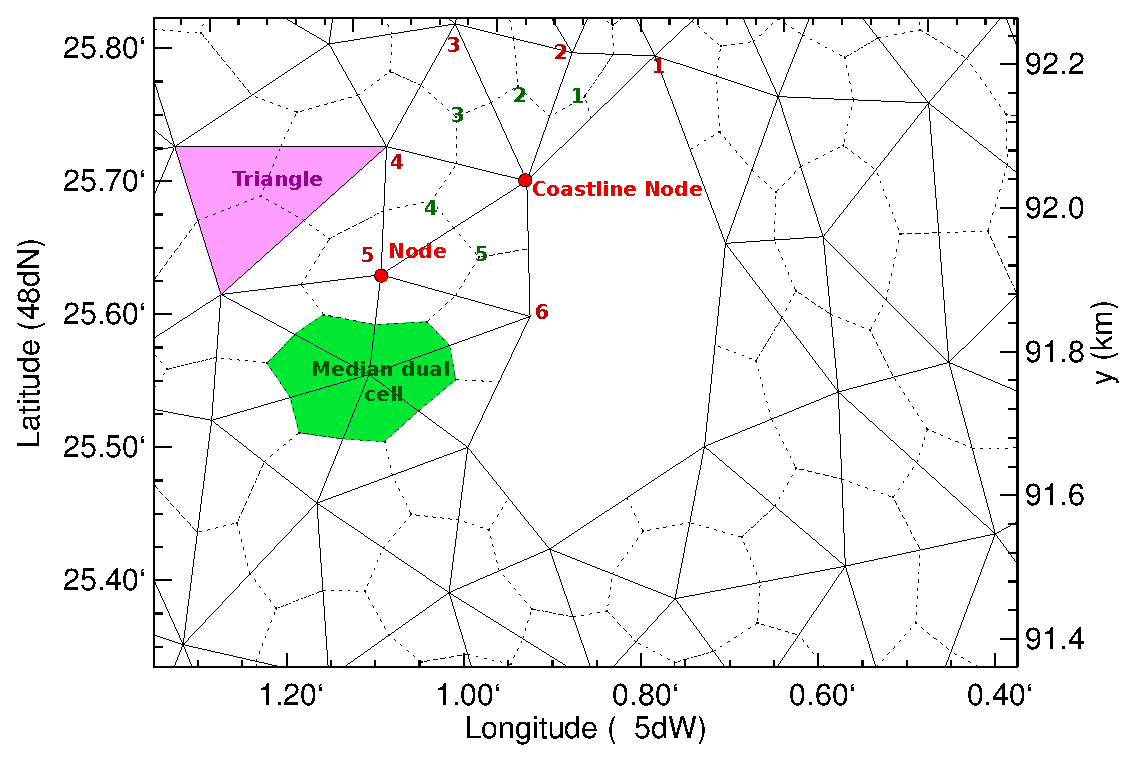
\epsfig{file=./num/grid_triangles.eps,angle=0,width=4.in}
\caption{Example of a region of a triangle-based mesh, with in this case the
 small Island of Bannec, France. If the depth is greater than the minimum
depth, the nodes of the shoreline are active. These are characterized by a
larger number of neighbor nodes (6 in the example chosen) than neighbor
triangles (5 in the same example).}
\label{fig:triangles} \botline
\end{center}
\end{figure}


\begin{figure} \begin{center}
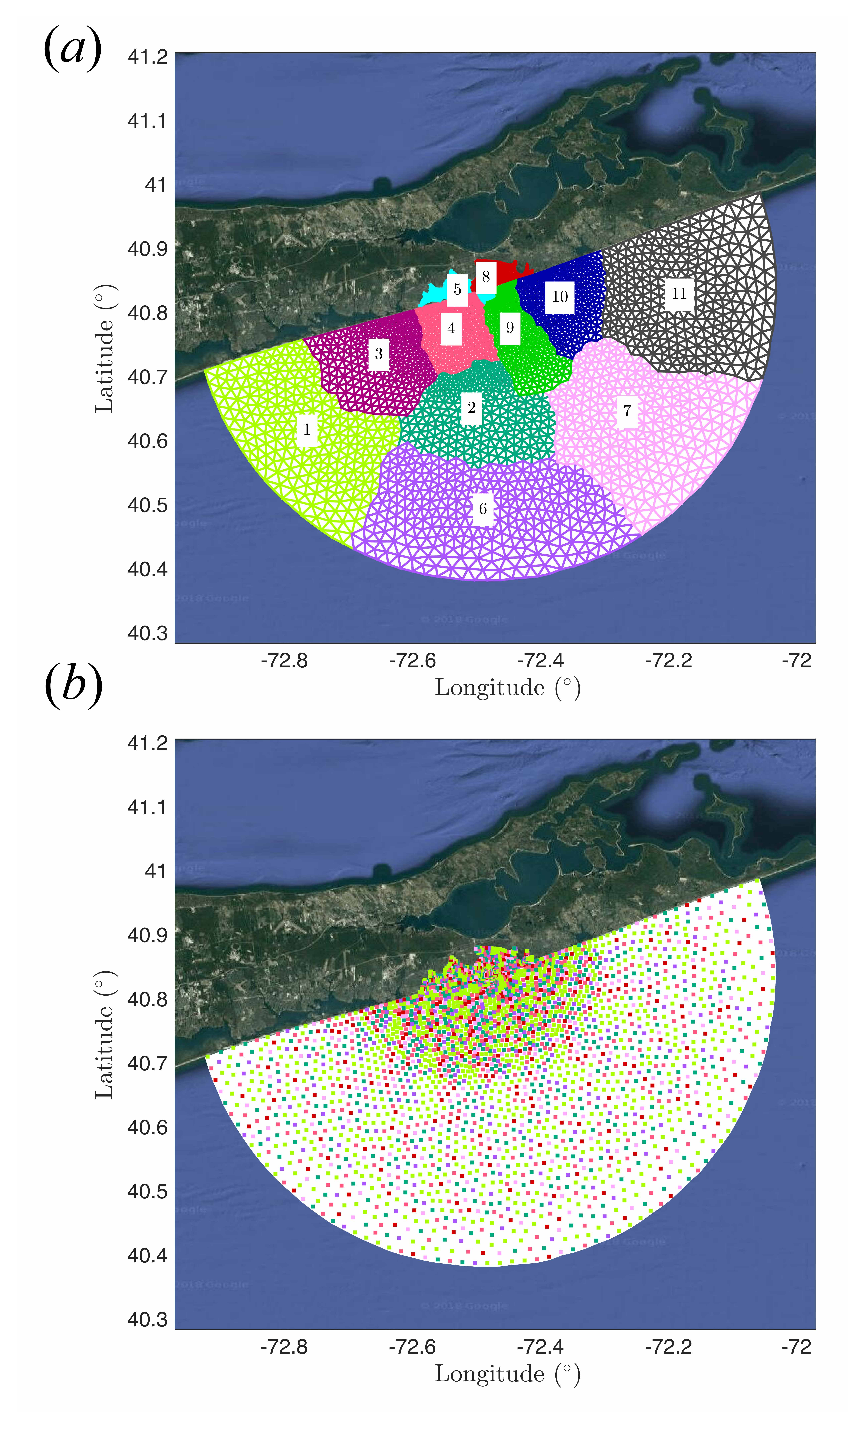
\epsfig{file=./num/DDvsCD.eps,angle=0,width=4.in}
\caption{The schematic difference between Domain Decomposition (a) and Card Deck approach (b) on 11 computational cores represented by colors. The grid has $\sim$3k nodes  and is build for Shinnecock Inlet, NY taken from an ADCIRC example problem.}
\label{DDvsCD} \botline
\end{center}
\end{figure}


\vssub
\subsubsection{~Spherical Multiple-Cell (SMC) grid} \label{sub:num_space_SMC}
\opthead{SMC}{\ws (MetOffice)}{J.-G. Li}

\noindent
The Spherical Multiple-Cell (SMC) grid \citep{art:Li11} is an extension of the 
Cartesian multiple-cell grid \citep{art:Li03} onto the spherical coordinate 
system. It is an unstructured grid but retains the conventional lat-lon grid 
cells so that all propagation formulations on the spherical coordinates are 
still applicable and hence all the finite difference schemes. The SMC grid 
relaxes the CFL restriction at high latitudes in a similar fashion as the 
reduced grid \citep{art:RA94}. Polar cells are introduced to remove the polar 
singularity of the differential transport equation by switching to an integral
equation. The upstream non-oscillatory 2nd order (UNO) advection schemes
\citep{art:Li08} is implemented on the SMC grid for both spatial and
inter-spectral propagation. The UNO2 scheme can be replaced with a 3rd order 
scheme using the {\F PSMC} namelist logical variable {\code UNO3}.  The UNO3 
scheme is similar to the UQ scheme but replacing its flux limiters with the 
UNO2 scheme.  A simple rotation scheme is used for wave refraction-induced 
rotation and the great circle turning \citep{art:Li12}.  The refraction scheme 
is unconditionally stable for any time step but the maximum refraction induced 
rotation angle is limited by the maximum possible refraction angle towards the 
local gradient direction.  Apart from this physical limiter, there is also a 
user-defined parameter {\code RFMAXD} in the {\F PSMC} namelist to limit the 
maximum refraction angle per time step.  Its default value is 36.0 degree.
Diffusion term similar to the \cite{art:BH87} for alleviation of the garden 
sprinkler effect is used but the diffusion coefficient is simplified to a 
single homogeneous parameter ($D_{nn}$ as in Eq.~(\ref{eq:Dnn_d})).  An 
additional 1-2-1 weighted averaging scheme is also available by the {\F PSMC} 
namelist logic variable {\code AVERG}.  Reduction of computing time with the 
SMC grid is significant in comparison with the conventional grid, thanks to the 
relaxed time step restriction at high latitudes and removal of land points from 
the model.  A remedy for the invalided scalar assumption at high latitude is 
provided to extend the global wave model into the entire Arctic Ocean 
\citep{art:Li16}.  This Arctic part can be activated by setting the {\F PSMC}
namelist parameter {\code Arctic=.TRUE.}.

The SMC grid can be used for replacing the regular lat-lon grid so that the
model domain can be extended to high latitudes or even the North Pole without
reducing the time step. This application requires few changes to the
regular grid model except for preparing a few extra input files, including the
cell array and face array files. The cell array can be generated with the
existing regular grid bathymetry by using the sea points only and merging
cells in the longitudinal directions at a few latitude steps \citep{art:Li11}.

Another important use of the SMC grid is for multi-resolution grids.
The base level SMC grid cell can be refined into 4 quarterly cells
by halving both the longitude and latitude grid lengths. Any cell
on this refined level can be further divided into another 4 quarterly
cells. This refinement can go on as required, resulting in multi-resolution
grids in a few refined levels. For consistency, the single resolution
SMC grid is considered to have only one level.  The normal regular grid input 
files, such as the water depth, land-sea masks, and sub-grid obstruction,
are no longer required, replaced with sea-point only cell and face arrays
and a sub-grid obstruction file.  The water depth is stored in the cell array 
in the last (5-th) column as an integer in meter.  The masks will be defined  
inside ww3\_grid with the sea-point cell array.

Wind and ocean current (if any) forcing can be applied using a regular grid at 
the base resolution as default input forcing for any SMC grid (single or multi-
level).  It will be interpolated on to the refined levels (if any) inside the 
model.  One option of sea-point only wind and current input for SMC grid can be 
switched on by the {\code SEAWND} logical variable in the {\F PSMC} namelist.  
This sea-point only option not only removes the need to interpolate the wind 
(and current, if any) inside the model but also allows different resolution 
wind (and current) forcing to be mixed up and interpolated to multi-resolution 
cells directly, making it a truly multi-resolution model. 

\begin{figure}
\centerline{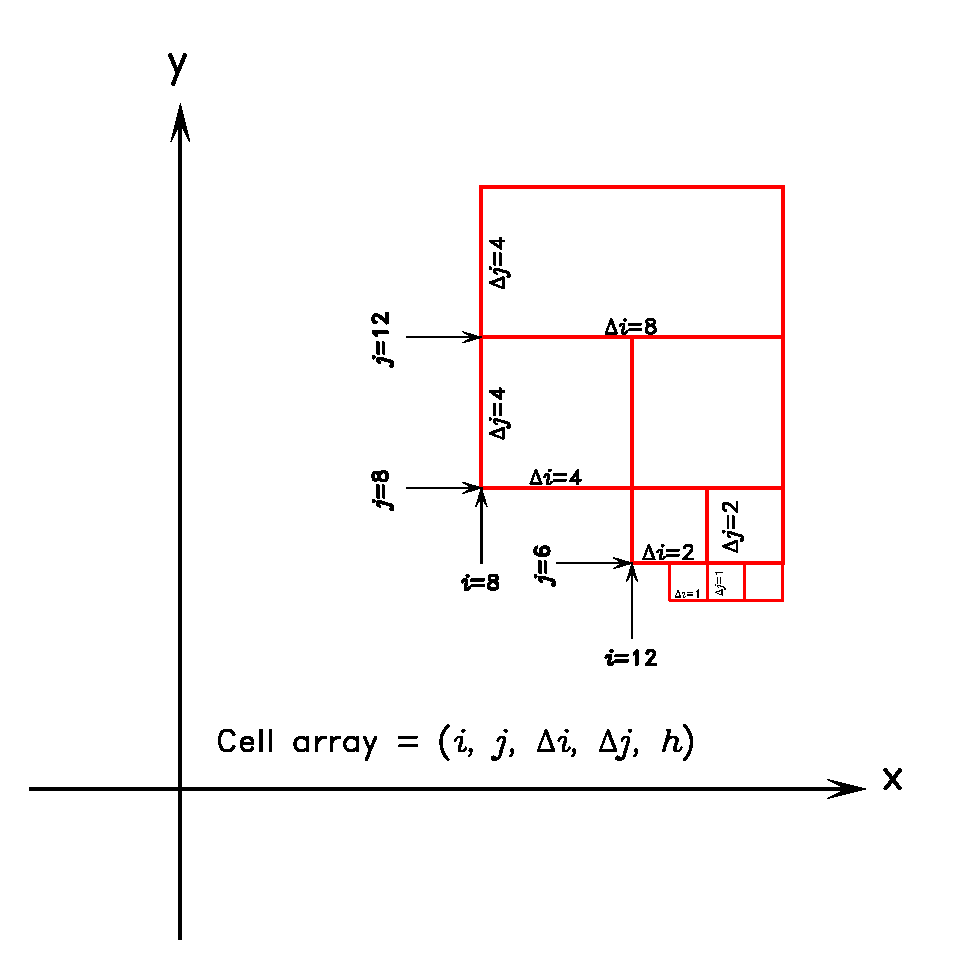
\epsfig{file=./num/smcelary.eps,angle=0,width=3.in}}
\caption{Illustration of cell arrays used in the SMC grid.}
\label{fig:SMCells} \botline
\end{figure}

One important feature of the SMC grid is that it is an unstructured grid, that
is, the cells are not required to be listed side by side as in their physical
position. For the convenience of multi-resolution SMC grid, the cells are
sorted by their sizes so that cells on one given level are grouped together in
one sub-loop for a shared sub-time-step.  The base level time step is halved
as the grid length for the refined level sub-step. This effectively avoids the
model to be slowed down by the refined cells due to their CFL restrictions. 
Neighbouring cells information for propagation schemes are provided with cell 
face arrays, which are pre-calculated for the given cell array list. So there 
is no need to expand the sea point only SMC grid cells onto a full grid for 
propagation. Fig.~\ref{fig:SMCells} illustrates how SMC cell arrays are 
defined and Fig.~\ref{fig:SMC_Arctic} shows the Arctic region in a 6-12-25 km 
three level SMC grid. The golden and red circles mark the global and Arctic 
parts in the SMC6-25 grid. The Arctic part within the golden circle requires a 
fixed reference direction to define its wave directional bins. The global part 
(up to the golden circle) can be run independently without the Arctic part. 
The 4 rows from the red to the golden circles are duplicated in the Arctic part 
as boundary cells if the Arctic part is activated with the ARC option.  
Separate cell and face arrays are used for the Arctic part and they are merged 
into the global ones within the wave model for propagation.  For a regional SMC
grid with input boundary conditions, a list of boundary cell sequential numbers
is required and the number of boundary cells is specified by the {\F PSMC}
namelist parameter {\code NBISMC}. The SMC grid uses boundary input file in the
same format as for a regular lat-lon grid.  The boundary file can be generated
with either a regular grid or a global SMC grid model by specifying the
boundary cell centre locations as for a regular grid.

\begin{figure}
\centerline{\epsfig{file=./num/JCP_Fig2_GArc.eps,angle=0,width=4.in}}
\caption{The Arctic region in a 6-12-25km multi-resolution SMC grid.}
\label{fig:SMC_Arctic} 
\botline
\end{figure}

Some IDL and F90 programs have been developed for generation of SMC grid cell
and face arrays and visualization of the grid mesh and wave fields but they
have not been formally included in the WW3 package yet. An IDL program 
(Glob50SMCels.pro) is provided in smc\_docs/SMCG\_TKs/ to generate a global 
50km SMC grid using a regular 50 km grid bathymetry file (G50kmBathy.dat). 
Face array generation is done with two F90 programs, one for the global part 
(G50SGlSide.f90) and one for the Arctic part (G50SAcSide.f90). Due to the 
special treatment of the polar cell \citep{art:Li12}, face arrays for the 
Arctic polar cell requires a different approach than other cells. The cell 
array file has to be sorted with a simple Linux script (countcells) before it 
is fed into the face array generation program.  The face arrays also need to be 
sorted with a Linux script (countijsd) to determine the multi-level sub-loop 
counts.  An independent spectral propagation test (G50SMCSRGD.f90) can be run 
to test the cell and face arrays and its output can be visualized with an IDL 
script, g50smstrspb.pro, which uses the saved projection files from the SMC 
grid visualization program, g50smcgrids.pro.  By modifying the projection 
parameters in g50smcgrids.pro, users can choose a projection view point (in 
lat-lon degree) and save the projection for model output visualization.  The 
sub-grid obstruction file can be generated with the idl program 
Glob50SMCObstr.pro.

Compilation of the SMC grid option is similar to that for the regular
lat-lon grid plus the extra switch {\code SMC} to invoke the SMC grid.  As SMC
grid shares some grid variables with the regular lat-lon grid, the regular grid
switches, such as {\code PR2 UNO} or {\code PR3 UQ} shoule be selected as well. 
The SMC grid type {\code SMCTYPE} is defined by replacing the {\code RECT} with
{\code SMCG} in the ww3\_grid.inp file.  Note that the SMC grid is built inside
the regular lat-lon grid so regular lat-lon grid parameters, such as NX, NY, 
SX, SY, X1, and Y1, are still required for a SMC grid in ww3\_grid.inp file at 
the base resolution level. The regular lat-lon grid water depth, land-sea 
masks, and sub-grid obstruction input files are no longer required and they are 
replaced with SMC grid sea point only files (depth is stored in the cell array 
and sub-grid obstruction in G50GObstr.dat).  The depth and land-sea mask input 
lines in ww3\_grid.inp are, however, kept for passing parameters, such as the 
minimum depth.  Due to the merges at high latitudes and refined resolutions if 
any, regular grid mapping arrays are modified slightly for consistency with the 
SMC grid cells.  Refer to the regression test \emph{regtests/ww3\_tp2.10}
for an example of a 3-level SMC grid model for the Lake Erie.

Output post processing for SMC grid models has been developed for
ww3\_ounf and ww3\_outf. For ww3\_ounf the user can choose between
retrieving multi-resolution information at native model grid sea-points,
or generating regular grids at any of the resolution levels set in
the model grid definition. The ww3\_outf program processes SMC grid data
as either the fully expanded regular lat-lon grid output at the base
resolution level or as ASCII output at all SMC grid sea-points (type-4).
For regular grid outputs, parameter values are determined
using an area-weighted average of all SMC grid cells overlapping the chosen
output cell boundaries. Sea-point data latitudes and longitudes 
correspond to the native model grid cell centres. For ww3\_ounf
sea-point outputs, variables describing cell sizes are also provided
in the netCDF file.

Visualization tools for sea-point outputs are not provided with this
code release; however, some examples are available from the Met Office
on request. For netCDF sea-point outputs a python based GUI tool has
been developed. Visualization of the all cell ASCII output can be done
with the aid of the input cell array file because the output cell 
sequence is the same as the input cell array. The IDL script 
g50smcswhglb.pro is an example program to plot the global 50km SMC grid
SWH output. It uses the projection files produced by g50smcgrids.pro. 
Users are encouraged to develop their own grid-generating and 
post-processing programs in other languages.  A Python group has formed to
develop SMC grid cell and face array generating and visualization programs.
These new Python programs are stored on a separate github site at present:  
\url{https://github.com/ww3-opentools/ww3-grid/}
which is still in its development stage.  WW3 Python programmers are welcome to
test and contribute for its improvement.  

The SMC grid is extended to run in the WW3 multi-grid mode from version 7.  At 
present, it only supports equal ranked SMC sub-grids to be run in parallel.
Generating of SMC sub-grids is similar for a single regional SMC grid with its
own boundary cell list.  It is recommended that the boundary cells are
duplicated cells from neighbouring sub-grids as boundary spectral exchanges for
SMC sub-grids are whole spectrum copy-paste, or no interpolation is required.
A regular lat-lon sub-grid could also be added to the same rank of the SMC 
sub-grid group but boundary condition will still be limited to whole spectral
exchange.  The original lat-lon grid boundary interpolation is not enabled. 
This simplification reduces MPI communication load but may lose some accuracy
if their boundary cell centres are not aligned.  See the regression test    
\emph{regtests/mww3\_test\_09} for an exmple of SMC sub-grids for the Great
Lakes.  It covers the Lake Michigan, Huron and Superior in 3 SMC levels 
(0.5-1-2 km) with minimized boundary links.
  
Hybrid parallelization is supported for SMC grids and it could reduce the total
elapsed time by half when it is run on the Cray XC40 supercomputer with 3 or 6
OpenMP threads. Further increase of OpenMP threads seems no much effect.  The 
combined hybrid and multi-grid parallelization may extend the computer usage
to over 100 nodes for the 3 Great Lake sub-grids in \emph{mww3\_test\_09}.

It is recommended to read the smc\_docs/SMC\_Grid\_Guide.pdf or the
conference paper \citep{tol:LiS17} at conference web page: 
http://www.waveworkshop.org/15thWaves/
for more information or to contact \url{Jian-Guo.Li@metoffice.gov.uk} 
for any help about the SMC grid.


\vsssub
\subsubsection{~The Garden Sprinkler Effect} \label{sub:num_GSE}
\vsssub

\noindent
The higher-order accurate propagation schemes are sufficiently free of
numerical diffusion for the so-called `Garden Sprinkler Effect' (GSE) to
occur, i.e., a continuous swell field disintegrates into a set of discrete
swell fields due to the discrete description of the spectrum
\citep[Fig.~3c]{art:BH87}. Several GSE alleviation methods are available in
\ws, as described in the following sections.

\addcontentsline{toc}{subsubsection}{\strut \hspace{24mm} No GSE alleviation}

\vspace{\baselineskip}
\vspace{\baselineskip}
\noindent {\bf No GSE alleviation}

\opthead{PR0 / PR1}{\ws}{H. L. Tolman}

\noindent
In case of no propagation (switch {\code PR0}) or for the first-order
propagation scheme in a traditional or curvilinear grid no GSE alleviation is
available or needed.
\pb
\addcontentsline{toc}{subsubsection}{\strut \hspace{24mm} Booij and Holthuijsen 1987}

\vspace{\baselineskip} 
\vspace{\baselineskip} 
\noindent {\bf Booij and Holthuijsen 1987}

\opthead{PR2}{\ws}{H. L. Tolman}


The classical GSE alleviation method is from \cite{art:BH87}, who derived an
alternative propagation equation for the discrete spectrum, including a
diffusive correction to account for continuous dispersion in spite of the
discrete spectral description. This correction influences spatial propagation
only, which for general spatial coordinates $(x,y)$ becomes

% ------ Correction linear dispersion --------- %
% eq:d_bal_0         Booij and Holthuijsen, 1987
% eq:Dxx
% eq:Dyy
% eq:Dxy
% eq:Dss
% eq:Dnn

\begin{equation}
\frac{\p \cN}{\p t} +
\frac{\p}{\p x} \left [ \dot{x} \cN 
           - D_{xx} \frac{\p \cN}{\p x} \right ] +
\frac{\p}{\p y} \left [ \dot{y} \cN 
           - D_{yy} \frac{\p \cN}{\p y} \right ] -
2 D_{xy} \frac{\p^2 \cN}{\p x \p y} = 0
\: , \label{eq:d_bal_0}\end{equation}  \begin{equation}
D_{xx} = D_{ss} \, \cos^2 \theta + D_{nn} \, \sin^2 \theta
\: , \label{eq:Dxx} \end{equation} \begin{equation}
D_{yy} = D_{ss} \, \sin^2 \theta + D_{nn} \, \cos^2 \theta
\: , \label{eq:Dyy} \end{equation}  \begin{equation}
D_{xy} = ( D_{ss} - D_{nn} ) \, \cos \theta \, \sin \theta
\: , \label{eq:Dxy} \end{equation} \begin{equation}
D_{ss} = (\Delta c_g )^2 \: T_s / 12
\: , \label{eq:Dss} \end{equation} \begin{equation}
D_{nn} =  ( c_g \Delta \theta )^2 \: T_s / 12
\: , \label{eq:Dnn} \end{equation}

\noindent
where $D_{ss}$ is the diffusion coefficient in the propagation direction of
the discrete wave component, $D_{nn}$ is the diffusion coefficient along the
crest of the discrete wave component and $T_s$ is the time elapsed since the
generation of the swell. In the present fractional step method the diffusion
can be added as a separate step

% eq:d_bal_1         Separated diffusion equation

\begin{equation}
\frac{\p \cN}{\p t} = 
\frac{\p}{\p x} \left [ D_{xx} \frac{\p \cN}{\p x} \right ] +
\frac{\p}{\p y} \left [ D_{yy} \frac{\p \cN}{\p y} \right ] +
   2 D_{xy} \frac{\p^2 \cN}{\p x \p y}
\: . \label{eq:d_bal_1} \end{equation}

\noindent
This equation is incorporated with two simplifications, the justification of
which is discussed in \cite{tol:OMB95}. First, the swell `age' $T_s$ is kept
constant throughout the model (defined by the user, no default value
available). Secondly, the diffusion coefficients $D_{ss}$ and $D_{nn}$ are
calculated assuming deep water

% eq:Dss_d
% eq:Dnn_d

\begin{equation}
D_{ss} = \left ( \: (X_\sigma-1) \: \frac{\sigma_m}{2 k_m} \right )^2
\: \frac{T_s}{12} \: , \label{eq:Dss_d} \end{equation} \begin{equation}
D_{nn} =  \left ( \frac{\sigma_m}{2 k_m} \Delta \theta \right )^2
\: \frac{T_s}{12} \: , \label{eq:Dnn_d} \end{equation}

\noindent
where $X_\sigma$ is defined as in Eq.~(\ref{eq:sigma_grid}). With these two
assumptions, the diffusion tensor becomes constant throughout the spatial
domain for each separate spectral component.

Equation~(\ref{eq:d_bal_1}) is solved using a forward-time central-space
scheme. At the cell interface between points $i$ and $i-1$ in $\phi$ ($x$)
space, the term in brackets in the first term on the right side of
Eq.~(\ref{eq:d_bal_1}) (denoted as $\cD_{i,-})$ is estimated as

% eq:ddif_1          Discrete diffusion 1

\begin{equation}
D_{xx} \frac{\p \cN}{\p x} \approx \cD_{i,-} =
\left . D_{xx} \; \left ( \frac{\cN_i - \cN_{i-1}}{\Delta x} \right ) \: 
\right |_{j,l,m} \: . \label{eq:ddif_1} \end{equation}

\noindent
Corresponding values for counters $i$ and $i+1$, and for gradients in
$\lambda$ ($y$) space again are obtained by rotating indices and
increments. If one of the two grid points is located on land,
Eq.~(\ref{eq:ddif_1}) is set to zero. The mixed derivative at the right side
of Eq.~(\ref{eq:d_bal_1}) (denoted as $\cD_{ij,--}$) is estimated for the grid
point $i$ and $i-1$ in $x$-space and $j$ and $j-1$ in $y$-space as

% eq:ddif_2          Discrete diffusion 2

\begin{equation}
\cD_{ij,--} = \left . \: D_{xy} 
\left ( \frac{- \cN_{i,j} + \cN_{i-1,j} +
              \cN_{i,j-1} - \cN_{i-1,j-1}}
           {0.5 ( \Delta x_j + \Delta x_{j-1} ) \: \Delta y}
              \right ) \: \right |_{l,m} 
\: . \label{eq:ddif_2} \end{equation}

\noindent
Note that the increment $\Delta x$ is a function of $y$ due to the use of the
spherical grid. This term is evaluated only if all four grid points considered
are sea points, otherwise it is set to zero. Using a forward in time
discretization of the first term in Eq.~(\ref{eq:d_bal_1}), and central in
space discretizations for the remainder of the first and second term on the
right side, the final algorithm becomes

% eq:ddif_3          Discrete diffusion 3

\begin{eqnarray}
\cN_{i,j,l,m}^{n+1} = \cN_{i,j,l,m}^n + 
\frac{\Delta t}{\Delta x} 
   \left ( \cD_{i,+} - \cD_{i,-} \right ) +
\frac{\Delta t}{\Delta y}
   \left ( \cD_{j,+} - \cD_{j,-} \right ) \nonumber \\
+ \frac{\Delta t}{4} \left ( \cD_{ij,--} + 
   \cD_{ij,-+} + \cD_{ij,+-} + \cD_{ij,++} \right )
\: . \label{eq:ddif_3} \end{eqnarray}

\noindent
Stable solutions are obtained for \citep[e.g.,][Part I section
7.1.1]{bk:Fle88}

% eq:ddif_4          Stability

\begin{equation}
\frac{D_{\max} \: \Delta t}{\min(\Delta x , \Delta y)^2}
\leq 0.5 \: , \label{eq:ddif_4} \end{equation}

\noindent
where $D_{\max}$ is the maximum value of the diffusion coefficient (typically
$D_{\max} = D_{nn}$). Because this stability criterion is a quadratic function
of the grid increment, stability can become a serious problem at high
latitudes for large scale applications. To avoid this putting undue
constraints on the time step of a model, a corrected swell age $T_{s,c}$ is
used

% eq:Ts_cor

\begin{equation}
T_{s,c} = T_s \min \left \{ \: 1 \: , \: 
\left ( \frac{\cos(\phi)}{\cos(\phi_c)} \right )^2 \: \right \}
\: , \label{eq:Ts_cor} \end{equation}

\noindent
where $\phi_c$ is a cut-off latitude defined by the user.

\vspace{\baselineskip} \noindent
 
The above diffusion is needed for swell propagation, but is not realistic
for growing wind seas. For wind seas, the \uq\ scheme without the
dispersion correction is sufficiently smooth to render stable fetch-limited
growth curves \citep{tol:OMB95}. To remove minor oscillations, a small
isotropic diffusion is used for growing wave components. To assure that this
diffusion is small and equivalent for all spectral components, it is
calculated from a preset cell Reynolds (or cell Peclet) number $\cR = c_g
\Delta x D_g^{-1} = 10$, where $D_g$ is the isotropic diffusion for growing
components

% eq:Dg              Diffusion growing components

\begin{equation}
D_g = \frac{c_g \: \min(\Delta x , \Delta y)}{\cR} \: . \label{eq:Dg}
 \end{equation}

\noindent
The diffusion for swell and for wind seas are combined using a linear
combination depending on the nondimensional wind speed or inverse wave age
$u_{10} c^{-1} = u_{10} k \sigma^{-1}$ as

% eq:Xg              Linear combination for diffusion
% eq:Dss_f           Final Dss
% eq:Dnn_f           Final Dnn

\begin{equation}
X_g = \min \: \left \{ \: 1 \: , \: \max \: \left [ \: 0 \: , \:
3.3 \left ( \frac{k \, u_{10}}{\sigma} \right ) - 2.3
\: \right ] \: \right \}
 \: , \label{eq:Xg} \end{equation} \begin{equation}
D_{ss} = X_g D_g + (1-X_g) D_{ss,p}
\: , \label{eq:Dss_f} \end{equation} \begin{equation}
D_{nn} = X_g D_g + (1-X_g) D_{nn,p}
\: , \label{eq:Dnn_f} \end{equation}

\noindent
where the suffix $p$ denotes propagation diffusion as defined in
Eqs.~(\ref{eq:Dss_d}) and (\ref{eq:Dnn_d}). The constants in Eqs~(\ref{eq:Dg})
and (\ref{eq:Xg}) are preset in the model.


\pb
\addcontentsline{toc}{subsubsection}{\strut \hspace{24mm} Spatial averaging}

\vspace{\baselineskip} 
\vspace{\baselineskip} 
\noindent {\bf Spatial averaging}

\opthead{PR3}{\ws}{H. L. Tolman}


The major drawback of the above GSE alleviation method is its potential impact
on model economy as discussed in relation to Eq.~(\ref{eq:ddif_4}) and in
\cite{tol:Waves01a,tol:OMOD02b}. For this reason, an alternative additional GSE alleviation
method has been developed for \ws.

This method which represents the default for \ws, replaces the
additional diffusion step (\ref{eq:d_bal_1}) with a separate fractional step
in which direct averaging of the field of energy densities for a given
spectral component is considered. The area around each grid point over which
the averaging is performed extends in the propagation ($\bs$) and normal
($\bn$) directions as

\begin{equation}
\pm \gamma_{a,s} \: \Delta c_g \: \Delta t \: \bs \:\:\: ,
\pm \gamma_{a,n} \: c_g \Delta \theta \: \Delta t \: \bn \:\:\: , \label{eq:GSE_avg}
\end{equation}

\noindent
where $\gamma_{a,s}$ and $\gamma_{a,n}$ are tunable constants, the default
value of which is set to 1.5. This averaging is illustrated in
Fig.~\ref{fig:GSE_1}. Note that these values may require some retuning for
practical applications, as discussed in \cite{tol:OMOD02b}. Appendix A of the
latter paper presents details of the averaging scheme, including conservation
considerations. Consistency with the \cite{art:BH87} approach furthermore
implies that $\gamma_{a,s}$ and $\gamma_{a,n}$ should vary with the spatial
grid resolution \citep[see][Appendix]{tol:OMOD08a}.

Note that this kind of averaging with dominant directions $\bs$ and $\bn$ is
similar to the \cite{art:BH87} diffusion method, that uses the same main
directions. The averaging method, however, never influences the time step,
because it is completely separated from the actual propagation. Moreover, if
explicit schemes are used with typically $c_g \Delta t / \Delta x < 1$, it is
obvious that the averaging over the area as defined in (\ref{eq:GSE_avg}) will
generally require information at directly neighboring spatial grid points
only, as in Fig.~\ref{fig:GSE_1}. Furthermore, this method does not require
high-latitude filtering.

\begin{figure} \begin{center}
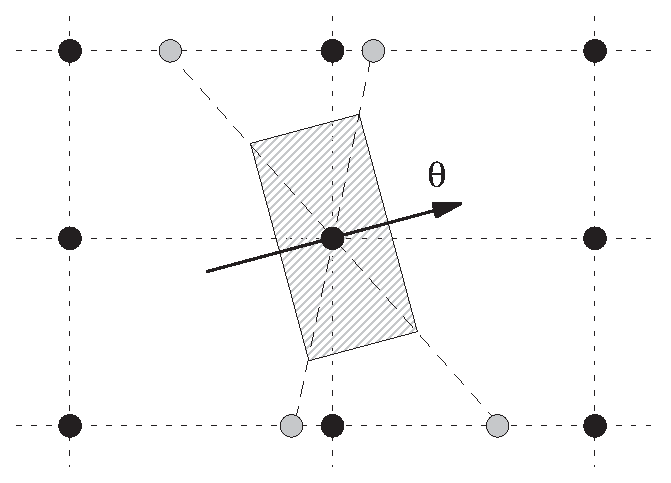
\epsfig{file=./num/GSE_1.eps,angle=0,width=2.2in}
\caption{Schematic of spatial averaging GSE alleviation technique. 
Solid circles and dotted lines represent the spatial grid. Hatched
area represent averaging area to be considered. Corner point values are
obtained from the central grid point and the gray points. The latter values
are obtained by interpolation from adjacent grid points
\citep[from][]{tol:OMOD02b}.}
\label{fig:GSE_1} \botline
\end{center}
\end{figure}

As is illustrated in \cite{tol:OMOD02b,tol:OMB02b}, this method gives
virtually identical results as the previous method, but does so at slightly
lower costs. For high-resolution applications, the averaging method may become
dramatically more economical.



Finally, the GSE can be alleviated somewhat by assuring that the discrete
spectral directions do not coincide with spatial grid lines. This can be
achieved by defining the first discrete direction $\theta_1$ as

% eq:theta1          First direction

\begin{equation}
\theta_1 = \alpha_\theta \: \Delta \theta \:\:\: , \label{eq:theta1}
\end{equation}

\noindent
where $-0.5 \leq \alpha_\theta \leq 0.5$ can be defined by the user. Note that
setting $\alpha \neq 0$ is beneficial to the first-order scheme, but has
negligible impact on the third-order scheme.
 

\pb
\vsssub
\subsubsection{~Unresolved obstacles} \label{sub:num_obst}
\conthead{\ws}{H. L. Tolman, L. Mentaschi}

\noindent
Even at the time of the original tuning of \ws\ version 1.15
\citep{tol:OMB02a}, it was clear that unresolved islands groups are a major
source of local wave model errors. This was illustrated in some more detail in
\citet[][Fig.~3]{tol:Waves01a}, and \citet[][Fig.~8]{tol:WaF02}. 
In \ws, two approaches are available for the parameterization
of unresolved obstacles. The first, originally from \swan\ \citep{art:BRH99,man:SWAN3},
applies the effects of unresolved obstacles at the cell boundaries of the spatial grid
within the numerical scheme, and is established for regular grids. 
The second approach, proposed by \citep{art:Mentaschi2015b}, is based on source terms,
and can be applied to different types of mesh.
In this section the first approach is presented, while for a description of the
second approach the reader is referred to section \ref{sec:UOST}.

In the propagation-based approach, the numerical fluxes between
cells through their common boundary are suppressed according to the degree of
obstruction provided by the unresolved obstacle. In this approach, the
numerical propagation scheme of the \uq\ scheme of Eq.~(\ref{eq:uq_xy_tot}) is
modified as

% eq:uq_xy_obstr

\begin{equation}
\cN_{i,j,l,m}^{n+1} = \cN_{i,j,l,m}^n +
\frac{\Delta t}{\Delta \phi} \left [ \alpha_{i,-} \cF_{i,-} - \alpha_{i,+} \cF_{i,+} \right ]
\: , \label{eq:uq_xy_obstr} \end{equation}

\begin{figure} \begin{center}
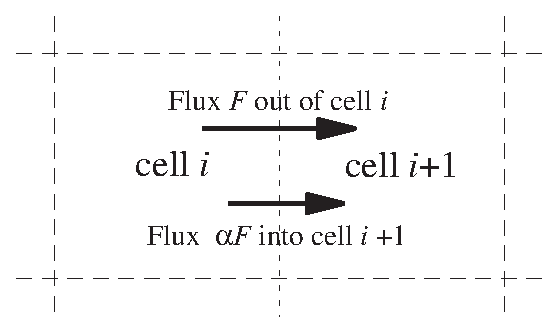
\epsfig{file=./num/obstr.eps,angle=0,width=2.2in}
\caption{Treatment of unresolved obstacles. Common cell
         boundary (dotted line) has transparency $\alpha$. Dashed lines
         represent other cell boundaries. Numerical flux from left to right.}
         \label{fig:obstr} \botline
\end{center}
\end{figure}

\noindent
where $\alpha_{i,-}$ and $\alpha_{i,+}$ are `transmissions' of the
corresponding cell boundaries, ranging from 0 (closed boundary) to 1 (no
obstructions). For outflow boundaries, transparencies by definition are 1,
otherwise energy will artificially accumulate in cells. For inflow boundaries,
transparencies less than 1 result in elimination of obstructed energy at the
cell boundary. This approach is illustrated in
Fig.~\ref{fig:obstr}. Note that a similar approach is easily adopted in the
first- and second-order schemes.  Note, furthermore, that an alternate
obstruction approach with obstructions as a function of the spectral direction
$\theta$ has been used by \cite{art:HY96} and \cite{art:HMM00}.

Two methods for defining the obstructions are available in the model. The
first defines the obstructions directly at the grid boundary. This requires
the generation of staggered depth-transparency grids. The second allows the
user to define depths and transparencies at the same grid. In this case, the
transparency at the inflow boundary becomes $0.5(1+\alpha_i)$, and the outflow
transparency by definition is 1. To complete the total transparency
$\alpha_i$, the next cell in the flow direction will have an inflow
transparency $2\alpha_i/(1+\alpha_i)$. If consecutive cells are partially
obstructed, the product of individual transparencies is applied.

This approach can also be used to continuously model the effects of ice
coverage on wave propagation. This is discussed in \para\ref{sub:num_ice}.
Details of the sub-grid treatment of islands and ice can be found in
\cite{tol:OMOD03a}. A study of impacts of this approach in large-scale wave
models is presented in \cite{tol:OMB02b,tol:OMOD03a}.

The default setting of \ws\ is to not include sub-grid modeling of
obstacles. Generating obstruction grids can be labor intensive. For this
reason, an automated approach for generating bottom and obstruction grids was
developed by \cite{tol:MMAB07a, tol:OMOD08a}.  Note that this option does not
involve compile-level choices, but is entirely controlled from the grid
preprocessor (see Chapter \ref{chapt:run}).


\vsssub
\subsubsection{~Continuously moving grids} \label{sub:num_move}
\opthead{MGx}{\ws}{H. L. Tolman}

\addcontentsline{toc}{subsubsection}{\strut \hspace{24mm} General concepts}


In order to address wave growth issues in rapidly changing, small scale
conditions such as hurricanes, an option to add a given continuous advection
speed to the grid has been added to the model in model version 3.02. This
model version is described in detail in \cite{tol:OMOD05b}. Here, only a
cursory description is given.



\begin{center}
\rule[1mm]{55mm}{1.0mm} WARNING \rule[1mm]{55mm}{1.0mm} \\
 \vspace{\baselineskip}
\parbox{120mm}{The continuously moving grid version of \ws\ is only intended 
for testing wave model properties in highly-idealized conditions. This model
version should only be used for deep water without mean currents and land
masses. Furthermore, to avoid complications with great circle propagation,
only a Cartesian grid should be used. The option is furthermore implemented only
for propagation options {\F pr1} and {\F pr3}. Note that this is not checked
in the scripts or programs at either the compile or run time level.  This
option is not considered to be for general application.} \\
\vspace{\baselineskip}
\rule[1mm]{55mm}{1.0mm} WARNING \rule[1mm]{55mm}{1.0mm}
\end{center}

\noindent
For the above described application Eq.~(\ref{eq:bal_plane}) can be written as

\begin{equation}
\frac{\partial N}{\partial t} + 
\left ( {\bf\dot{x}}-{\bf{v}}_g \right ) \cdot \nabla_x N  = 
\frac{S}{\sigma} \: , \label{eq:bal_move}
\end{equation}

\noindent
where ${\bf{v}}_g$ represents the advection velocity of the grid. This option
is selected when compiling the model. A second compile level
option allows for adding the grid advection velocity ${\bf{v}}_g$ to the wind
field. This allows for a simple method to assure mass conservation of a wind
field independent of the actual and instantaneous grid advection velocity. The
advection velocity ${\bf{v}}_g$ can vary in time and is provided by the user
at the run time of the model (see below).




For the simplified conditions for which Eq.~(\ref{eq:bal_move}) is valid, the
implementation of the moving grids is trivial if it is considered that this
equation is equivalent to

\begin{equation}
\frac{\partial N}{\partial t} + 
\nabla_x \cdot \left ( {\bf\dot{x}}-{\bf{v}}_g \right ) N  = 
\frac{S}{\sigma} \: , \label{eq:bal_move2}
\end{equation}

\noindent
which in turn implies that the advection velocity ${\bf{v}}_g$ can be added
directly to ${\bf\dot{x}}$ for arbitrary numerical schemes solving
Eq.~(\ref{eq:bal_plane}). Because this influences the net advection velocity,
it also influences stability characteristics. This impact has been accounted
for automatically by including the moving grid velocity in the calculation of
the actual propagation time step in Eq~(\ref{eq:dtpl}). Hence, the user need
to provide a proper maximum propagation time step representative for $\bf{v}_g
= 0$ only.

The motion of the grid has an apparent influence on the Garden Sprinkler
Effect (GSE), due to the different retention time in the grid of spectral
components with identical frequency but different propagation direction.
Current GSE alleviation methods tend to be more efficient for younger swells
than for older swells. Hence, swells with longer retention time in the moving
grid tend to show a more pronounced GSE \citep[see][]{tol:OMOD05b}. To
mitigate this apparent imbalance in GSE alleviation,  Eq.~(\ref{eq:GSE_avg}) is
replaced with

\begin{equation}
\pm \gamma_a \gamma_{a,s} \: \Delta c_g \: \Delta t \: \bs \:\:\: ,
\pm \gamma_a \gamma_{a,n} \: c_g \Delta \theta \: \Delta t \: \bn \:\:\: ,
\label{eq:move_GSE_avg1}
\end{equation}

\begin{equation}
\gamma_a = \left ( \frac{|\dot{\bf{x}}|}{|\dot{\bf{x}}-\bf{v}_g|}
\right ) ^{p}
\label{eq:move_GSE_avg2}
\end{equation}

\noindent
where $\gamma_a$ is a correction factor accounting for the grid movement, and
where the power $p$ is a parameter allows for some tuning. With this
modification, the effects of the GSE can be distributed more evenly over the
grid by rescaling the amount of smoothing applied with the expected residence
time of corresponding spectral component in the moving grid
\citep[see][]{tol:OMOD05b}.


To switch on the moving grid option or the corrections of the wind field or GSE, three
optional switches are added to the \ws\ source code (also see, \para\ref{sec:switches}:

\begin{slist}
\sit{mgp} {Apply advection correction for continuous moving grid.}
\sit{mgw} {Apply wind correction for continuous moving grid.}
\sit{mgg} {Apply GSE alleviation for
           continuous moving grid.}
\end{slist}

\noindent
The advection velocity and direction is input to the shell similar to the
input of homogeneous currents (see bottom of file {\file ww3\_shel.inp} in
Section~\ref{sec:ww3shel}), exchanging the keyword `{\code CUR}' with `{\code
  MOV}'. The advection velocity can be changed in time like all homogeneous
input fields. An example of running with a moving grid model is given in test
case {\file ww3\_ts3}. A similar capability exist in {\file ww3\_multi.inp} in
Section \ref{sec:ww3multi}, and is tested in test case {\file mww3\_test\_05}.

\vssub
\subsubsection{~Rotated grids} \label{sub:num_space_rotagrid}
\opthead{RTD}{\ws\ (MetOffice)}{J.-G. Li}

\noindent
The rotated grid is a latitude-longitude (lat-lon) grid and is obtained by
rotating the North Pole to a new position at latitude $\phi_{p}$ and
longitude $\lambda_{p}$ in the standard latitude-longitude system.  The new
pole position is chosen so that the model domain of interest may be placed
around the rotated equatorial area for a evenly-spaced lat-lon mesh. For this
reason the rotated grid is also known as \emph{Equatorial grid}. For instance,
the North Atlantic and European wave (NAEW) model used in the UK Met Office
uses a rotated pole at 37.5N, 177.5E so that London, UK
(\textasciitilde{}51.5N 0.0E) is almost on the rotated equator. This rotated
grid allows a much more evenly spaced lat-lon mesh in the NAEW domain than the
standard lat-lon grid in the same area. 

In \ws\, the rotated grid is implemented with minimum changes to the original
lat-lon grid. In fact, the rotated grid is treated just like the standard 
lat-lon grid inside the model. To set up and run a rotated grid model configuration,
users should choose the regular lat-lon grid along with the {\code RTD} switch.
The rotated pole position is set using the {\code PLAT} and {\code PLON} variables in the
{\bf ww3\_grid.inp} namelist {\code ROTD}. Model input files, like wind, current and ice files 
should be mapped on to the rotated grid. For convenience of nesting in standard 
lat-lon grid frameworks, boundary conditions provided to and output from the 
rotated grid use spectra referenced to a standard grid north and standard lat-lon
grid points values, which are converted into rotated grid lat-lon inside \ws\.
The list of 2D spectral output locations in {\bf ww3\_shel.inp} are also specified in 
standard lat-lon. 

Model directional and x-y vector outputs can be converted to a standard grid
north reference by setting the UNROT variable in the {\bf ww3\_grid.inp} namelist
ROTD to True. With this set, for point outputs lat-lon locations all directional
values such as wind direction, current direction and 2D spectra are converted
into standard lat-lon orientation. Functions to de-rotate gridded
fields are applied in {\bf ww3\_ounf}, {\bf ww3\_outf} and {\bf ww3\_grib}. 
When running {\bf ww3\_ounf} and {\bf ww3\_ounp}, the resulting netCDF
files will include a variable attribute direction\_reference, which describes
whether a standard (True North) or rotated grid directional reference frame
has been used. Gridded netCDF files generated by {\bf ww3\_ounf} also include
\emph{standard\_latitude} and \emph{standard\_longitude} two-dimensional arrays
that describe location of the rotated model cell centres in the standard lat-lon
reference frame. 

Six subroutines are provided in module {\bf w3servmd.ftn} for rotated grid
conversion:
\begin{vlist}
\vit{w3spectn}{}{Turns wave spectrum anti-clockwise by AnglD}
\vit{w3acturn}{}{Turns wave action(k,nth) anti-clockwise by AnglD}
\vit{w3thrtn}{}{Turns direction parameters anti-clockwise by AnglD}
\vit{w3xyrtn}{}{Turns x-y vector parameters anti-clockwise by AnglD}
\vit{w3lltoeq}{}{Convert standard into rotated lat/lon plus AnglD}
\vit{w3eqtoll}{}{Reverse of w3lltoeq, but AnglD unchanged}
\end{vlist}
These subroutines are self-contained and can be extracted outside the model
for pre- or post-processing of rotated grid files.  Some conversion tools have
been developed based on these subroutines but have not been included in \ws\
yet. Refer to the regression test \emph{regtests/ww3\_tp2.11} for an example
of a rotated grid model (NAEW).  Users may find more information in
\emph{smc\_docs/Rotated\_Grid.pdf} or contact Jian-Guo Li for help
(\url{Jian-Guo.Li@metoffice.gov.uk}).

\vssub
\subsection{~Intra-spectral propagation} \label{sub:spec}
\vssub
\subsubsection{~General concepts}
\vsssub

The third step of the numerical fractional step algorithm considers refraction
and residual (current-induced) wavenumber shifts. Irrespective of the spatial
grid discretization and coordinate system, the equation to be solved in this
step becomes

%-----------------------------------%
% Step : Intra-spectral propagation %
%-----------------------------------%
% eq:step_intra
% eq:k_dot_g

\begin{equation}
\frac{\p N}{\p t} + \frac{\p}{\p k} \, \dot{k}_g N +
\frac{\p}{\p \theta} \, \dot{\theta}_g N = 0
\: , \label{eq:step_intra} \end{equation} \begin{equation}
\dot{k}_g  = \frac{\p \sigma}{\p d} 
    \frac{{\bf U} \cdot \nabla_x d}{c_g}  -
    {\bf k} \cdot \frac{\p {\bf U}}{\p s}
\: , \label{eq:k_dot_g} \end{equation}

\noindent
where $\dot{k}_g$ is the wavenumber velocity relative to the grid, and
$\dot{\theta}_g$ is given by (\ref{eq:theta_g_dot}) and (\ref{eq:theta_dot}).
This equation does not require boundary conditions in $\theta$-space, as the
model by definition uses the full (closed) directional space. In $k$-space,
however, boundary conditions are required. At low wavenumbers, it is assumed
that no wave action exists outside the discrete domain. It is therefore
assumed that no action enters the model at the discrete low-wavenumber
boundary. At the high-wavenumber boundary, transport across the discrete
boundary is calculated assuming a parametric spectral shape as given by
Eq. (\ref{eq:tail_N_k}). The derivatives of the depth as needed in the
evaluation of $\dot{\theta}$ are mostly determined using central
differences. For points next to land, however, one-sided differences using sea
points only are used.

Propagation in $\theta$-space can cause practical problems in an explicit
numerical scheme, as the refraction velocity can become extreme for long waves
in extremely shallow water or due to strong current shears. Similarly, 
the propagation in $k$-space suffers from similar problems in very shallow water. 
To avoid the need of extremely small time steps
due to refraction, the propagation velocities in $\theta$-space and $k$-space
(\ref{eq:theta_dot}) are filtered,

% eq:theta_filter

\begin{equation}
\dot{\theta} = X_{rd}(\lambda,\phi,k)\left( \dot{\theta_d} + 
\dot{\theta_c} + \dot{\theta_g} \right)\: , \label{eq:theta_filter} \end{equation}

\noindent
where the indices $d$, $c$ and $g$ refer to the depth, current and great-circle
related fraction of the refraction velocity in (\ref{eq:theta_dot}). The
filter factor $X_{rd}$ is calculated for every wavenumber and location
separately, and is determined so that the \cfl\ number for propagation in
$\theta$-space due to the {\em depth} refraction term cannot exceed a pre-set
(user defined) value (default 0.7). This corresponds to a reduction of the
bottom slope for some low frequency wave components. For mid-latitudes, the
affected components are expected to carry little energy because they are in
extremely shallow water. Long wave components carrying significant energy are
usually traveling toward the coast, where their energy is dissipated
anyway. This filtering is also important for short waves, and close to the
pole. The effect of this filter can be tested by reducing the time steps for
intraspectral refraction and by looking at the maximum CFL numbers in the
output of the model.  These are computed just before the filter is applied.

% \vspace{\baselineskip}
% \centerline{\ldots ADD DYNAMIC TIME INTEGRATION \ldots}


The spectral space is always discretized with constants directional increments
and a logarithmic frequency grid (\ref{eq:sigma_grid}) to accommodate
computations of the nonlinear interaction $S_{nl}$. First, second and third
orders schemes are available, and are presented in the following sections.
\vssub
\subsubsection{~First-order scheme}
\opthead{PR1}{\ws}{H. L. Tolman}

\noindent
In the first order scheme the fluxes in $\theta$- and $k$-space are calculated
using Eqs. (\ref{eq:1up_xy_1}) through (\ref{eq:1up_xy_3}) (replacing $\cN$ with
$N$ and rotating the appropriate counters). The complete first order scheme
becomes

% eq:1up_intra_tot

\begin{equation}
N_{i,j,l,m}^{n+1} = N_{i,j,l,m}^n 
 + \frac{\Delta t}{\Delta \theta} \left [ \cF_{l,-} - \cF_{l,+} \right ]
 + \frac{\Delta t}{\Delta k_m} \left [ \cF_{m,-} - \cF_{m,+} \right ]
\: , \label{eq:1up_intra_tot} \end{equation}

\noindent
where $\Delta \phi$ is the directional increment, and $\Delta k_m$ is the
(local) wavenumber increment. The low-wavenumber boundary conditions is
applied by taking $\cF_{m,-}=0$ for $m=1$, and the high wavenumber boundary
condition is calculated using the parametric approximation (\ref{eq:tail_N_k})
for $N$, extending the discrete grid by one grid point to high wavenumbers.
\vssub
\subsubsection{~Second-order scheme (UNO)}
\opthead{UNO}{Met Office}{J.-G. Li}

\noindent
The UNO scheme for the directional $\theta$-space is identical to the regular
grid one assuming that the directional bins are regularly spaced. For the
\emph{k}-space, however, the UNO scheme uses its irregular version, which
uses local gradients instead of differences to estimate wave action value at
the mid-flux point for the cell face between spectral bin \emph{i}-1 and
\emph{i}, that is:
\begin{equation}
  N_{i-}^{*}=N_{c}+sign\left(N_{d}-N_{c}\right)\frac{\left(\Delta
      k_{c}-|\dot{k}_{i-}|\Delta
      t\right)}{2}\min\left(|\frac{N_{u}-N_{c}}{k_{u}-k_{c}}|,|\frac{N_{c}-N_{d}}{k_{c}-k_{d}}|\right)
  \:\:\:,
\label{eq:UNO2irregular}
\end{equation}

\noindent
where \emph{i}- is the wave number \emph{k} bin index; the subscripts
\emph{u}, \emph{c} and \emph{d} indicate the \emph{upstream, central} and
\emph{downstream} cells, respectively, relative to the given \emph{i}- face
velocity $\dot{k}_{i-}$; $k_{c}$ is the central bin wave number and $\Delta
k_{c}$ is the central bin widith. Details of the irregular grid UNO scheme are
given in \cite{art:Li08}.

Boundary conditions for the $\theta$-space is the natural periodic
condition. For the \emph{k}-space, two more zero spectral bins are added to
each end of the wave spectral domain as the UNO scheme is 2nd order in
accuracy.



\vssub
\subsubsection{~Third-order scheme (UQ)}
\opthead{UQ}{\ws}{H. L. Tolman}

\noindent
The \uq\ scheme for the $\theta$-space is implemented similar to the scheme
for physical space, with the exception that the closed direction space does
not require boundary conditions. The variable grid spacing in $k$-space
requires some modifications to the scheme as outlined by
\cite[{Appendix}]{art:Leo79}. Equations~(\ref{eq:quick_1}) through
(\ref{eq:quick_4}) then become

% ------ QUICKEST scheme for k space---------- %
% eq:quick_1k        Basic flux
% eq:quick_2k        Boundary value
% eq:quick_3k        Divergence
% eq:quick_4k        CFL number

\begin{equation}
\cF_{m,-} = \left [ \dot{k}_{g,b} \: N_b \: \right ]^n_{i,j,l}
\: , \label{eq:quick_1k}\end{equation} \begin{equation}
\dot{k}_{g,b} = 0.5 \: \left ( \dot{k}_{g,m-1} + \dot{k}_{g,m} 
\: \right )  \: , \label{eq:quick_1ak}
\end{equation} \begin{equation}
N_b = \frac{1}{2} \left [ \rule[0mm]{0mm}{\baselineskip} \: 
(1+C)N_{i-1} + (1-C)N_i \: \right ] - \:
\frac{1-C^2}{6} \: {\cal CU} \: \Delta k^2_{m-1/2}, \label{eq:quick_2k} \end{equation} \begin{equation}
{\cal CU} =  \left \{ \begin{array}{ccc}
\frac{1}{\Delta k_{m-1}}
\left [ \frac{N_{ m }-N_{m-1}}{\Delta k_{m-1/2}} - 
        \frac{N_{m-1}-N_{m-2}}{\Delta k_{m,-3/2}} \right ]
               & \mbox{for} & \dot{k}_b \geq 0 \\
\frac{1}{\Delta k_m}
\left [ \frac{N_{m+1}-N_{ m }}{\Delta k_{m+1/2}} -
       \frac{N_{ m }-N_{m-1}}{\Delta k_{m-1/2}} \right ]
               & \mbox{for} & \dot{k}_b   <  0
\end{array} \right . \: , \label{eq:quick_3k}
\end{equation} \begin{equation}
C = \frac{\dot{k}_{g,b} \: \Delta t}{\Delta k_{m-1/2}}
\: , \label{eq:quick_4k} \end{equation}

\noindent
where $\Delta k_m$ is the discrete band or cell width at grid point $m$, and
where $\Delta k_{m-1/2}$ is the distance between grid points with counters $m$
and $m-1$. The \ult\ limiter can be applied as in Eqs.~(\ref{eq:ult_1})
through (\ref{eq:ult_4}), if the \cfl\ number of Eq.~(\ref{eq:quick_4k}) is
used. At the low- and high-wavenumber boundaries the fluxes again are
estimated using a first-order upwind approach, with boundary conditions as
above defined for the first-order scheme. The final scheme in $k$-space
becomes

% eq:1uq_k_tot

\begin{equation}
N_{i,j,l,m}^{n+1} = N_{i,j,l,m}^n 
 + \frac{\Delta t}{\Delta k_m} \left [ \cF_{m,-} - \cF_{m,+} \right ]
\: , \label{eq:uq_k_tot} \end{equation}
\vssub
\subsection{~Non-ice source term integration} \label{sub:source}
\vssub

The source terms not involving ice are accounted for by solving

%---------------------%
% Step : Source terms %
%---------------------%
% eq:step_source

\begin{equation}
\frac{\p N}{\p t} = \cS_{no~ice} \: . \label{eq:step_source}
\end{equation}

\noindent 
As in \wam, a semi-implicit integration scheme is used. In this scheme the
discrete change of action density $\Delta N$ becomes \citep{art:WAM88}

% eq:implicit_st

\begin{equation}
\Delta N(k,\theta) = \frac{\cS(k,\theta)}{1- \epsilon D(k,\theta)\Delta t}
\: , \label{eq:implicit_st} \end{equation}

\noindent 
where $D$ represents the diagonal terms of the derivative of $\cS$ with
respect to $N$ \citep[Eqs. 4.1 through 4.10]{art:WAM88}, and where $\epsilon$
defines the offset of the scheme. Originally, $\epsilon = 0.5$ was implemented
to obtain a second-order accurate scheme. Presently, $\epsilon = 1$ is used because it is more appropriate for the large time steps in the equilibrium range of
the spectrum \citep{pro:HA98,art:HA01} and it results in much smoother
integration of the spectrum. The change of $\epsilon$ has little impact on
mean wave parameters, but makes the dynamical time stepping as described below
more economical.

The semi-implicit scheme is applied in the framework of a dynamic
time-stepping scheme \citep{tol:JPO92}. In this scheme, integration over the
global time step $\Delta t_g$ can be performed in several dynamic time steps
$\Delta t_d$, depending on the net source term $\cS$, a maximum change of
action density $\Delta N_m$ and the remaining time in the interval $\Delta
t_g$. For the $n^{\rm th}$ dynamic time step in the integration over the
interval $\Delta t_g$, $\Delta t_d^n$ is calculated in three steps as

% ------ Dynamic s.t. int. scheme ------- %
% eq:st_d_1
% eq:st_d_2a
% eq:st_d_2b
% eq:st_d_3

\begin{equation}
\Delta t_d^n = 
\min_{f<f_{hf}} \left [ \frac{\Delta N_m}{|\cS|}
\left ( 1 + \epsilon D \frac{\Delta N_m}{|\cS|} \right ) ^{-1}
\right ] \: , \label{eq:st_d_1}
\end{equation} \begin{equation}
\Delta t_d^n = \max \: \left [ \: \Delta t_d^n \: , \: 
\Delta t_{d,\min} \right ] \: , \label{eq:st_d_2a}
\end{equation} \begin{equation}
\Delta t_d^n = \min \: \left [ \: \Delta t_d^n \: , \: 
\Delta t_g - \sum_{i=1}^{n-1} \Delta t_d^i
 \: \right ] \: , \label{eq:st_d_2b}
\end{equation}

\noindent
where $\Delta t_{\min}$ is a user-defined minimum time step, which is added to
avoid excessively small time steps. The corresponding new spectrum $N^n$
becomes

\begin{equation}
N^n = \max\: \left [ \: 0 \: , \: N^{n-1} + 
\left ( \frac{\cS \Delta t_d}{1 - \epsilon D \Delta t_d} \right )
\: \right ] \: . \label{eq:st_d_3}
\end{equation}


The maximum change of action density $\Delta N_m$ is determined from a
parametric change of action density $\Delta N_p$ and a filtered relative
change $\Delta N_r$

% eq:st_d_4
% eq:st_d_5
% eq:st_d_6
% eq:st_d_7

\begin{equation}
\Delta N_m (k,\theta) = \min \: \left [ \:
\Delta N_p (k,\theta) \: , \: \Delta N_r (k,\theta) 
\: \right ] \: , \label{eq:st_d_4}
\end{equation} \begin{equation}
\Delta N_p (k,\theta) = X_p \: \frac{\alpha}{\pi} \:
\frac{(2\pi)^4}{g^2} \: \frac{1}{\sigma k^3}
\: , \label{eq:st_d_5}
\end{equation} \begin{equation}
\Delta N_r (k,\theta) = X_r \; \max \: \left [ \: 
N(k,\theta) \: , \: N_f \: \right ] \: , \label{eq:st_d_6}
\end{equation} \begin{equation}
N_f = \max \: \left [ \: \Delta N_p (k_{\max},\theta) \: , 
\: X_f \: \max_{\forall k,\theta} \left \{ N(k,\theta) \right \}
\: \right ] \: , \label{eq:st_d_7} \end{equation}

\noindent 
where $X_p$, $X_r$ and $X_f$ are user-defined constants (see
Table~\ref{tab:st_d_p}), $\alpha$ is a {\sc pm} spectrum energy level (set to $\alpha =
0.62\times 10^{-4}$) and $k_{\max}$ is the maximum discrete wavenumber. The
parametric spectral shape in (\ref{eq:st_d_5}) corresponds in deep water to
the well-known high-frequency shape of the one-dimensional frequency spectrum
$F(f) \propto f^{-5}$. The link between the filter level and the maximum
parametric change in (\ref{eq:st_d_7}) is used to assure that the dynamic time
step remains reasonably large in cases with extremely small wave energies. A
final safeguard for stability of integration is provided by limiting the
discrete change of action density to the maximum parametric change
(\ref{eq:st_d_5}) in conditions where Eq.~(\ref{eq:st_d_2a}) dictates $\Delta
t_d^n$. In this case Eq.~(\ref{eq:st_d_2a}) becomes a limiter as in the WAM
model. Impacts of limiters are discussed in detail in for instance
\cite{art:HJ99,art:HJ01}, \cite{art:HA01} and \cite{tol:GAOS02}.

% tab:st_d_p

\begin{table} 
\begin{center} \begin{tabular}{|l|c|c|c|c|} \hline \hline
                 & $X_p$     & $X_r$             & $X_f$ &
$\Delta t_{d,\min}$      \\ \hline
\wam\ equivalent & $\frac{\pi}{24}10^{-3}\Delta t$
 & $\infty (\geq 1)$ & --    & $\Delta t_g$  \\ 
 suggested       & 0.1-0.2  & 0.1-0.2 & 0.05 & $\approx 0.1 \Delta t_g$ \\  
default setting  &  0.15    &   0.10  & 0.05 & -- \\ \hline \hline
\end{tabular} \end{center}
\caption{User-defined parameters in the source term integration
 scheme}
\label{tab:st_d_p} \botline \end{table}

The dynamic time step is calculated for each grid point separately, adding
additional computational effort only for grid points in which the spectrum is
subject to rapid change. The source terms are re-calculated for every dynamic
time step.

It is possible to compile \ws\ without using a linear growth term. In such a
case, waves can only grow if some energy is present in the spectrum. In
small-scale applications with persistent low wind speeds, wave energy might
disappear completely from part of the model. To assure that wave growth can
occur when the wind increases, a so-called seeding option is available in \ws\
(selected during compilation). If the seeding option is selected, the energy
level at the seeding frequency $\sigma_{\rm seed} = \min(\sigma_{\max}, 2\pi
f_{hf})$ is required to at least contain a minimum action density

% ------ Spectral seeding ------- %
% eq:seed

\begin{eqnarray}
N_{\min}(k_{seed},\theta) & = & 
        6.25 \times 10^{-4} \frac{1}{k_{\rm seed}^3 \: \sigma_{\rm seed}}
        \max \left [ \: 0. \: , \: \cos^2 ( \theta - \theta_w ) \right ]
                             \nonumber \\ & & \hspace{5mm}
        \min \left [ \: 1 \: , \: \max \left ( \: 0 \: , \: 
        \frac{|u_{10}|}{X_{\rm seed} g \sigma_{\rm seed}^{-1}}-1 
\: \right ) \: \right ] \: , \label{eq:seed} \end{eqnarray}

\noindent
where $g \sigma_{\rm seed}^{-1}$ approximates the equilibrium wind speed for
the highest discrete spectral frequency. This minimum action distribution is
aligned with the wind direction, goes to zero for low wind speeds, and is
proportional to the integration limiter (\ref{eq:st_d_5}) for large wind
speeds. $X_{\rm seed} \geq 1$ is a user-defined parameter to shift seeding to
higher frequencies. Seeding starts if the wind speed reaches $X_{\rm seed}$
times the equilibrium wind speed for the highest discrete frequency, and
reaches its full strength for twice as high wind speeds. The default model
settings include the seeding algorithm, with $X_{\rm seed} = 1$.

In model version 3.11, surf-zone physics parameterizations have been
introduced. Such physics, particularly depth-induced breaking, operate on much
smaller time scales than deep water and limited-depth physics outside the surf
zone. To assure reasonable behavior for larger time steps, an additional
optional limiter has been adopted from the SWAN model, which can be used instead of 
modeling surf-breaking explicitly.  This limiter is similar to the Miche
style maximum wave height in the depth-limited wave breaking source term of
Eq.~(\ref{eq:BJ78_Miche}). In this limiter, the maximum wave energy $E_m$ is
computed as

% ------ Surf zone limiter ------ %
% eq:MLIM

\begin{equation}
E_m = \frac{1}{16} [ \gamma_{lim}  \tanh ( \bar{k} d ) / \bar{k} ] ^2
\:\:\: , \label{eq:MLIM} 
\end{equation}

\noindent
where $\gamma_{lim}$ is a factor comparable to $\gamma_M$ in
Eq.~(\ref{eq:BJ78_Miche}), with the caveat that $\gamma_M$ is representative
for an individual wave, whereas $\gamma_{lim}$ is representative for the
significant wave height. For monochromatic waves, the original expression by
\cite{art:Miche44} would correspond to $\gamma_{lim} = 0.94$ and replacing
$H_s$ by the height $H$ of the waves. Here this idea is applied to random
waves.  In shallow water, this limits $H_s$ to be less than $\gamma_{lim} d$.
If the total spectral energy $E$ is larger than the maximum energy $E_m$, the
limiter is applied by simply rescaling the spectrum by the factor $E/E_m$,
loosely following the argumentation from \cite{art:EB96} and used
in \para\ref{sec:DB1}.  

This limiter can be switched on or off in the
compilation of the model, and $\gamma_{lim}$ can be adjusted by the user. The
default is set to $\gamma_{lim} = 1.6$ because $H_{rms}$ values close to $d$
have indeed been recorded and thus taking a ratio $H_s/H_{rms}$ of 1.4, using
1.6 allows this large steepness to be exceeded by some margin.  Note that this
limiter should be used as a `safety valve' only, and hence that it should be
less strict than the breaking criterion in the surf-breaking or whitecapping
source terms, if these source terms are modeled explicitly.

Also, this limiter does not guarantee that all parts of the spectrum are
realistic. Indeed, the use of a mean wavenumber, as in the Komen et
al. dissipation, makes it possible to have unrealistically steep short waves
in the presence of swell. A future extension of this limiter could be to limit
the steepness with a partial spectral integration in frequencies, to make sure
that waves of all scales are indeed not too steep.

\vssub
\subsection{~Ice source terms integration} \label{sub:icesource}
\vssub

Because the attenuation and scattering in the ice can be very strong (although they are linear), it is convenient 
to perform a separate integration of the ice terms $S_{\mathrm{ice}}=S_{\mathrm{id}}+S_{\mathrm{is}}$. This combines 
a dissipation term 
\begin{equation}
S_{\mathrm{id}}/\sigma  = \beta_{\mathrm{id}} N ,
\end{equation}
 and a scattering term 
which is of the form 
\begin{equation}
 \frac{S_{\mathrm{is}}(k,\theta)}{\sigma} =  \int_0^{2\pi}\beta_{\mathrm{is}} [N(k,\theta')-N(k,\theta)] d\theta'  ,
 \end{equation}
 in which the scattering coefficient $\beta_{\mathrm{is}}$ is a priori a function of the difference in direction between 
 incident $\theta'$ and scattered $\theta$ directions, as well as the shape of ice floes. In general 
  the directional spectrum $N(k,.)$ is a vector with {\F NTH} (number of directions) components, 
and the source term is a vector of the same size  given by the matrix product $S/\sigma = M N(k,.)$ where  
$M$ is a positive symmetric square {\F NTH} by {\F NTH} matrix with components given from the $\beta_{\mathrm{id}}$ values.
The matrix $M$ is easily diagonalized as 
\begin{equation}
 M  =  V D V^T  ,
 \end{equation}
 where $D$ is a diagonal matrix containing all eigenvalues and $V$ is the array of eigenvectors, 
 and $V^T$ is its transpose. As a result the split wave action equation for ice source terms 
 \begin{equation}
\frac{\p}{\p t} \frac{N}{c_g}   = \frac{S_{\mathrm{id}}}{\sigma c_g} ,
 \end{equation}
 can be rewritten for the action $N_i$ of each eigenvector $V_i$ with eigenvalue $\lambda_i$ as 
  \begin{equation}
\frac{\p}{\p t} \frac{N_i}{c_g}   = \frac{\beta_{\mathrm{id}} + \lambda_i}{\sigma c_g} N_i ,
 \end{equation}
 which has the following exact solution 
   \begin{equation}
 {N_i}(t+\Delta t_g)   = N_i(t) \exp \left[ (\beta_{\mathrm{id}} + \lambda_i) +\Delta t_g\right].
 \end{equation}
 
 In all cases the eigenvector corresponding to an isotropic spectrum has an eigenvalue $\lambda=\beta_{\mathrm{id}}$. 
 In the case of an isotropic back-scatter, the other eigenvalues are all equal to $(\beta_{\mathrm{id}} + \beta_{\mathrm{is}})$. 
 This decomposition over the two eigenspaces simplifies the solution to 
%---------------------%
% Step : Source terms %
%---------------------%
% eq:exact_st_ice
\begin{equation}
 N(t+\Delta t_g) = \exp(\beta_{\mathrm{id}} \Delta t_g) \overline{N}(t)  + \exp \left[\left(\beta_{\mathrm{id}} + \beta_{\mathrm{is}}\right) \Delta t_g\right] \left[N(t)-\overline{N}(t)\right]
, \label{eq:exact_st_ice} \end{equation}
where $\overline{N}$ is the average over all directions. As a result, for a spatially homogeneous field, 
the spectrum exponentially tends to isotropy over a time scale $1/(\beta_{\mathrm{id}})$.

\vssub
\subsection{~Simple ice blocking ({\code IC0})} \label{sub:num_ice}
\opthead{IC0}{\ws}{H. L. Tolman} %\conthead{\ws}{H. L. Tolman}

\noindent
Ice covered sea is considered as `land' in \ws, assuming zero wave energy and
boundary conditions at ice edges are identical to boundary conditions at shore
lines. Grid points are taken out of the calculation if the ice concentration
becomes larger than a user-defined concentration. If the ice concentration
drops below its critical value, the corresponding grid point is
`re-activated'. The spectrum is then initialized with a PM spectrum based on
the local wind direction with a peak frequency corresponding to the
second-highest discrete frequency in the grid. A low energy spectrum is used to
assure that spectra are realistic, even for shallow coastal points.

The above discontinuous ice treatment represents the default model setting in
\ws. In the framework of the modeling of unresolved obstacles as discussed in
\para\ref{sub:num_obst}, a continuous method is also available, as given by
\cite{tol:OMOD03a}. In this method, a user-defined critical ice concentration
at which obstruction begins ($\epsilon_{c,0}$) and is complete
($\epsilon_{c,n}$) are given (defaults are $\epsilon_{c,0} = \epsilon_{c,n} =
0.5$, i.e., discontinuous treatment of ice). From these critical
concentrations, corresponding decay length scales are calculated as

\begin{equation}
l_0 = \epsilon_{c,0} \min ( \Delta x , \Delta y )
, \label{eq:l0}
\end{equation}
\begin{equation}
l_n = \epsilon_{c,n} \min ( \Delta x , \Delta y )
, \label{eq:ln}
\end{equation}

\noindent
from which cell transmissions in $x$ and $y$ ($\alpha_x$ and $\alpha_y$,
respectively) are calculated as

\begin{equation}
\alpha_x = \left \{ \begin{array}{ccl}
 1 & \mbox{for} & \epsilon \Delta x < l_0 \\
 0 & \mbox{for} & \epsilon \Delta x > l_n \\
\frac{l_n - \epsilon \Delta x}{l_n - l_0} & \multicolumn{2}{c}{\mbox{otherwise}} 
\end{array} \right .
\:\:\: , \:\:\:
\alpha_y = \left \{ \begin{array}{ccl}
 1 & \mbox{for} & \epsilon \Delta y < l_0 \\
 0 & \mbox{for} & \epsilon \Delta y > l_n \\
\frac{l_n - \epsilon \Delta y}{l_n - l_0} & \multicolumn{2}{c}{\mbox{otherwise}} 
\end{array} \right .
\:\:\: . \label{eq:ice_0} 
\end{equation}

\noindent
Details of this model can be found in \cite{tol:OMOD03a}.

Updating of the ice map within the model takes place at the discrete model
time approximately half way in between the valid times of the old and new ice
maps. The map will not be updated, if the time stamps of both ice fields are
identical.

The above description pertains to the switch {\code IC0}. Note that either ice transmissions for propagation ({\code IC0}), or ice as a source term can be used ({\code IC1}, {\code IC2}, {\code IC3}), but not both approaches at the same time.

\vssub
\subsection{~Winds and currents} \label{sub:num_w_c}
\vssub

\noindent
Model input mainly consists of wind and current fields. Within the model,
winds and currents are updated at every time step $\Delta t_g$ and represent
values at the end of the time step considered. Several interpolation methods
are available (selected during compilation). By default, the interpolation in
time consists of a linear interpolation of the velocity and the direction
(turning the wind or current over the smallest angle). The wind speed or
current velocity can optionally be corrected to (approximately) conserve the
energy instead of the wind velocity. The corresponding correction factor $X_u$
is calculated as

% eq:X_u10

\begin{equation}
X_u = \max \left [ \: 1.25 \: , \: \frac{u_{10,rms}}{u_{10,l}}
\right ] \: , \label{eq:X_u10} \end{equation}

\noindent
where $u_{10,l}$ is the linearly interpolated velocity and $u_{10,rms}$ is the
rms interpolated velocity. Finally, winds can optionally be kept constant and
changed discontinuously (option not available for current).

Note that the auxiliary programs of \ws\ include a program to pre-process
input fields (see \para\ref{sec:ww3prep}). This program transfers gridded
fields to the grid of the wave model. For winds and currents this program
utilizes a bilinear interpolation of vector components. This interpolation can
be corrected to (approximately) conserve the velocity or the energy of the
wind or the current by utilizing a correction factor similar to
Eq.~(\ref{eq:X_u10}).

\vssub
\subsection{~Use of tidal analysis} \label{sub:num_tide}
\conthead{\ws}{F. Ardhuin}

\noindent
In order to reduce the volume of input files, the water levels and currents
can be defined by their tidal amplitudes and phases. This is made possible by
using the {\code TIDE} switch which activates the detection of the needed
information in current.ww3 and level.ww3 files. The tidal analysis can be
performed from NetCDF current or water level files, using the {\file
  ww3\_prnc} preprocessing program. In that case the analysis method uses the
flexible tide analysis package by \cite{art:For09}. The precomputed tidal constituents 
can be used at run time by {\file ww3\_shel}.

However, that method may not be very efficient due to the large memory 
required to store a large number of tidal constituents because, like other 
forcing parameters, they are not decomposed across processors: each processor stores the full 
spatial grid of forcing parameters. To avoid this,  
the tidal constituents can be used to generated time series with the tidal
prediction program {\file ww3\_prtide}, which produces the usual {\file current.ww3} or 
{\file level.ww3} files.

The choice of tidal constituents for the analysis and prediction are specified
in the input files for {\file ww3\_prnc} and {\file ww3\_prtide}. Two
short-cuts are defined. {\code VFAST} is the following selection of 20
components, Z0 (mean), SSA, MSM, MSF, MF, 2N2, MU2, N2, NU2, M2, S2, K2, MSN2,
MN4, M4, MS4, S4, M6, 2MS6, and M8. When using {\code ww3\_shel} to do the
tidal prediction, the time step for currents or water is set to 1800~s.

In {\file ww3\_prtide}, there is also a quality check on the values of the
tidal constituents that is performed: unrealistically large values of the
amplitudes for some constituents can be defined in {\file ww3\_prtide.inp}.
For model grid points where these are exceeded, all components are set to
zero, except for UNST grids, in which the neighbors are searched to provide a
reasonable value and avoid strong gradients.

\vssub
\subsection{~Wave crest and height space-time extremes} \label{sub:space_time_ext}
\conthead{\ws (ISMAR, NCEP)}{Barbariol, F., Benetazzo, A., Alves, J.H.G.M.}

Space-Time (ST) extreme waves are modeled in WAVEWATCH III based on the Euler Characteristics (EC) approach, which states that for a given multi-dimensional (2-D space + time), statistically homogeneous and stationary Gaussian random wave field, the probability of exceedance of the maximal sea surface elevation is approximated by means of the mean value of the EC \citep{Fed12eu}. The ST extreme elevation model used here was formulated by \cite{Fed12sp} for Gaussian sea waves, and extended to second-order nonlinear spatial wave fields by \cite{Fed13} and spatio-temporal fields by \cite{Beet15}. The proposed ST extreme linear model was assessed with numerical simulations \citep{Baet15,Baet16}, while the extension to second-order nonlinear waves was verified using stereo imaging \citep{Fed13,Beet15}. According to those models, the probability of exceedance of the second-order nonlinear ST maximal crest height $\eta_{2ST_m}$ is approximated (for large threshold $z_2$ with respect to the standard deviation of the surface elevation $\sigma$) as:
\begin{equation}
P(\eta_{2ST_m} > z_2) \approx \left[N_{3D} \left( \frac{z_1}{\sigma} \right)^{2} + N_{2D} \left( \frac{z_1}{\sigma} \right) + N_{1D} \right] \exp{ \left( -\frac{z_1^2}{2 \sigma^2} \right)},
\label{eq_STE1}
\end{equation}
where the nonlinear threshold $z_2$ is related to its linear approximation $z_1$ via the Tayfun quadratic equation using the steepness parameter $\mu$, strictly valid in deep waters, which accounts for bandwidth effects. Parameters $N_{3D}$, $N_{2D}$, and $N_{1D}$ express the average number of 3D, 2D, and 1D waves within the ST region, respectively, and are determined from the moments $m_{ijl}$ of the directional wave spectrum $S(k, \theta)$ defined as follows:
\begin{equation}
m_{ijl}=\int k_{x}^{i}k_{y}^{j}\omega^{l}S(k,\theta)dkd\theta.
\label{eq_STE2}
\end{equation}

The average number of waves in Eq. (\ref{eq_STE1}) also depends on the size of the spatio-temporal domain, namely the spatial dimension $X$ along the mean direction of wave propagation, the spatial dimension $Y$ orthogonal to the mean direction of wave propagation, and the duration $D$. The expected value $\bar{\eta}_{2ST_m}$ (output parameter \textbf{STMAXE}, in meters) of the random variable $\eta_{2ST_m}$ is given by
\begin{multline}
\bar{\eta}_{2ST_m}=\mathbb{E}\left\{\eta_{2ST_m} \right\} = \\ 
	\sigma \left[(h_1+\frac{\mu}{2}h_1^{2})+
\gamma \left( h_1-\frac{2N_{3D}h_1+N_{2D}}{N_{3D} h_1^{2}+N_{2D} h_1+N_{1D}}\right)^{-1} (1+\mu h_1) \right],
\label{eq_STE3}
\end{multline}
where $\gamma \approx 0.5772$ is the Euler-Mascheroni constant, and $h_1$ is the dimensionless (with respect to the standard deviation $\sigma$) most probable (mode) extreme value, which is the largest solution of the implicit equation in $h$
\begin{equation}
\left[N_{3D} h^{2} + N_{2D} h + N_{1D} \right] \exp{ \left( -\frac{h^2}{2} \right)}=1.
\label{eq_STE4}
\end{equation}

The standard deviation $\sigma_{2_m}$ (output parameter \textbf{STMAXD}, in meters) of the crest height $\eta_{2ST_m}$ is given by:
\begin{equation}
\sigma_{2_m}=std(\eta_{2ST_m})=\sigma \frac{\pi}{\sqrt{6}} \left( h_1-\frac{2N_{3D}h_1+N_{2D}}{N_{3D} h_1^{2}+N_{2D} h_1+N_{1D}}\right)^{-1} (1+\mu h_1) .
\label{eq_STE5}
\end{equation}

The expected value of the ST extreme crest-to-trough wave height is obtained using the Quasi-Determinism (QD) model, which predicts the mean shape of ST wave groups close to the apex of their development. According to the QD model the expected value of the crest-to-trough height $\bar{H}_{1_{cm}}$ (output parameter \textbf{HCMAXE}, in meters) of the wave with linear extreme crest height $\bar{\eta}_{1ST_m}$ is expressed as
\begin{equation}
\bar{H}_{1_{cm}}=\mathbb{E}\left\{H_{1_{cm}} \right\} = \bar{\eta}_{1ST_m}(1-\psi_1^* / \sigma^2),
\label{eq_STE6}
\end{equation}
where $\psi_1^* < 0$ is the value of the first minimum of the temporal autocovariance function computed from the spectrum as
\begin{equation}
\psi_1(\tau) = \int S(\omega) \cos{(\omega \tau)} d \omega,
\label{eq_STE7}
\end{equation}
and $\bar{\eta}_{1ST_m}  \psi_1^*/\sigma^2 < 0$ is the expected displacement of the wave trough preceding or following the expected linear extreme crest height $\bar{\eta}_{1ST_m}$, which is computed using Eq. (\ref{eq_STE3}) after letting the wave steepness $\mu=0$. For a given linear group, the height $\bar{H}_{1_{cm}}$ is generally smaller than the maximum expected wave height $\bar{H}_{1_m}$ (output parameter \textbf{HMAXE}, in meters), which is computed as
\begin{equation}
\bar{H}_{1_m}=\mathbb{E}\left\{H_{1_m} \right\} = \bar{\eta}_{1ST_m}\sqrt{2(1-\psi_1^* / \sigma^2)}.
\label{eq_STE8}
\end{equation}

The effect on wave heights of second-order nonlinearities is generally small, particularly in narrow band seas, and it will be neglected in the present implementation to reduce the computational cost. Uncertainty of estimates of $\bar{H}_{1_{cm}}$ (output parameter \textbf{HCMAXD}, in meters) and $\bar{H}_{1_m}$ (output parameter \textbf{HMAXD}, in meters) are determined using the standard deviation of $\eta_{1ST_m}$ ($\sigma_{1_m}$, which is computed using Eq. (\ref{eq_STE5}) after letting the wave steepness $\mu=0$) as follows:
\begin{eqnarray}
std({H}_{1_m})&=&\sigma_{1_m}\sqrt{2(1-\psi_1^* / \sigma^2)}, \nonumber \\
std({H}_{1_{cm}})&=&\sigma_{1_m}(1-\psi_1^* / \sigma^2).
\label{eq_STE9}
\end{eqnarray}

To activate the computation of wave crest and height space-time extremes in WAVEWATCH III, the user has to specify values of the {\F MISC} namelist parameters {\code STDX}, {\code STDY} and {\code STDT} in {\file ww3\_grid.inp} different to -1 (the latter is a default value that avoids computer overheads when these parameters are not wanted). {\code STDX} and {\code STDY} are spatial dimensions over which extremes are calculated. {\code STDT} is the time length over which extremes are calculated. If {\code STDX} and {\code STDY} are left at default values (-1), but {\code STDT} has a namelist value different to default (e.g., greater than 0), then extreme values are provided over time, for a point. Conversely, if {\code STDT} is kept at default (-1) and {\code STDX} and {\code STDY} are greater than zero, instantaneous extreme values are computed over space. When all three parameters are greater than zero, space-time probabilities and values are computed.

Wave crest and height space-time extremes outputs follow the standard WAVEWATCH III parameter framework, and have to be specified as namelists or flags in {\file ww3\_shel.inp} or {\file ww3\_multi.inp}, in which case they are included in the standard gridded binary output files during a model run. Consequently, they also have to be specified in gridded output post-processors for obtaining a final human-readable form. Space-time extremes output parameters available in WAVEWATCH III are provided in Table \ref{tab:ste_parm}.

\begin{table}[h]
\begin{center} \begin{tabular}{|l|c|c|} \hline \hline
Internal Label & User-Interface Label & Description \\ \hline
STMAXE  &   MXE   & Max surface elev (STE) \\
STMAXD  &   MXES  & STD of max crest (STE) \\
HMAXE   &   MXH   & Max wave height (STE) \\
HCMAXE  &   MXHC  & Max wvhgt from crest (STE) \\
HMAXD   &   SDMH  & STD of MXH (STE) \\
HCMAXD  &   SDMHC & STD of MXHC (STE) \\ \hline
\end{tabular}
\end{center}
\caption{User-defined parameters in the computation of wave crest and height space-time extremes.}
\label{tab:ste_parm} \botline \end{table}



\vssub
\subsection{~Spectral partitioning} \label{sub:num_part}
\conthead{APL Wave / XWaves / IMEDS}{B. Tracy, C. Bunney}

The sea-states predicted by numerical wave models are often complex, due to the
presence of multiple wave trains formed as a result of both local wind action and
more distant storms. In order to better describe these local wind-sea and remote
swell components, without dealing with the full complexity of the model wave spectrum,
the spectrum can be partitioned into collections of spectral bins from which more
recognisable wave statistics (height, period, direction) can be derived. 

\noindent
Fig. \ref{fig:partitions} shows an example surface plot of an energy density
spectrum at one grid point at a specific time.  The amount of energy density
at each frequency-direction intersection is shown by this surface.  The
surface is divided into shaded areas or partitions representing energy from
sub-peaks within the spectrum.  Fig. \ref{fig:partitions} shows four
spectral partitions, an area of windsea and three swell trains.  The total
energy represented by this spectrum can be defined by bulk parameters, such as
the significant wave height $H_s$. The shaded areas, called partitions of the
spectrum, show spectral sub-features that give more information about this
grid point's energy situation.  \ws\ has point and field output options
available to provide quantitative descriptions of these individual spectral
partition such as partition wave height, peak period of partition (parabolic
fit), peak wavelength of partition, mean direction of partition, wind-sea
fraction of partition ($W$) using Eq.~(\ref{eq:wsf}), and the number of
partitions.  In the field output, these parameters correspond to spectral partitioned output fields 
\ref{out:first_part} through \ref{out:last_part} and can be found in
\para\ref{sub:outpars}.

Across the wave forecasting community, various methods of spectral partitioning
and definition of waves as sea or swell have been adopted. Two varieties of partitioning
are available from the W3PARTMD module.
\begin{enumerate}
  \item Topographic partitioning that groups spectral bins together into (multiple) 
        distinct wave systems.
  \item A simple frequency based cutoff that produces two partitions; one above
        and one below a cutoff frquency.
\end{enumerate}
The topographic partitioning methods in \ws\ are all based on a watershedding technique
using the original partitioning code implemented by B. Tracey (see below). These are
further categorised according to the method by which a partition is determined to be
either wind-sea or swell. The cutoff methods are varied dependent upon whether the
user chooses to use a set frequency (e.g. to delineate between high frequency sea waves 
and lower frequency swells) or allows the threshold to vary according to the
local wind speed and direction.

\subsubsection{Topographic partitioning method}

Since the two-dimensional spectrum in Fig.~\ref{fig:partitions} looks like a
topological surface, it is logical to apply an image processing partitioning
algorithm that treats the spectral surface like a topographical surface.  The
partitioning shown in Fig.~\ref{fig:partitions} is based on a digital image
processing watershed algorithm \citep{art:VS91} first prototyped by
\cite{pro:HJ04} for the analysis of ocean wave data. 
The US continental divide where everything to the east goes into the Atlantic
Ocean and everything to the west goes into the Pacific Ocean is a typical
example of a watershed line.  The oceans represent minima that determine the
watershed line.  If the spectral surface is inverted, the spectral peaks
become catchments and watershed lines or partition boundaries can be
determined using the \cite{art:VS91} algorithm.  Calculation of parameters for
each spectral partition can then be accomplished and wave system analysis as
described in \cite{art:HP01} can be applied.  \cite{pro:HJ04} and
\cite{tol:Vict06b} used a MATLAB code to apply the \cite{art:VS91}
algorithm\footnote{~Now available as XWaves from
http://www.WaveForceTechnologies.com, replacing the previous APL WAVES
package}.  This code has been transformed to an efficient FORTRAN routine for
use in \ws since version 3.11.  Coding follows the
\cite{art:VS91} paper but incorporates an efficient sort routine (O(n))
discussed in \cite{rep:TTH06}.

\begin{figure} \begin{center}
\epsfig{file=./num/partition1.eps,width=3.8in}
\caption{Surface plot of an energy density spectrum showing spectral
         partitions for windsea and three swell trains.  This is a snapshot of
         hindcasted conditions at Christmas Island (NOAA buoy 51028) at
         12:00~UTC on November 9, 2000.}
         \label{fig:partitions} \botline
\end{center}
\end{figure}

\subsubsection{Sea/swell assignment and partitioning method}

The second stage in the partitioning process is the assignment of individual
partitions to (wind-)sea and swell categories in point or field outputs. In the
default option for \ws\ these comprise a single wind-sea (partition 1) and a set
of swell components ordered by wave height. Selecting alternative partition methods
changes the categorisation as described below. 

The partitioning method is set in the MISC namelist in ww3\_grid.inp via the PTM parameter:
\begin{itemize}

 \item PTM=1: Wind sea and swells defined using topographic partitions and
   		  classified using a wind sea fraction cutoff (WWIII default scheme).
		  Outputs wind-sea plus swell 1,2,3 etc.

 \item PTM=2: Wind sea and swells defined using topographic partitions and
          spectral wave-age cutoff. Outputs wind-sea plus swell 1,2,3 etc.
		  
 \item PTM=3: Wave components defined using topographic partitions only. Outputs partitions
          ranked by wave height as partition 1,2,3 etc.

 \item PTM=4: Wind sea and swell defined using spectral wave-age cutoff. Outputs wind-sea and single swell partition.

 \item PTM=5: Wave components defined using a user defined frequency cutoff (PTFCUT).
        Outputs high frequency and low frequency partition.
\end{itemize}

In PTM1, topographic partitions for which the percentage of wind-sea energy exceeds a 
defined fraction are aggregated and assigned to the wind-sea component (e.g., the first
partition). The remaining partitions are assigned as swell components in order of 
decreasing wave height.

PTM2 works in a very similar way to PTM1, by first identifying a primary wind-sea component,
which is assigned as the first partition, then a number of swell (or secondary wind-sea) 
partitions are identified, as follows. A set of secondary spectral partitions is established 
using the topographic method, each partition is checked in turn, with any of their spectral 
bins influenced by the wind (based on a wave age criterion) being removed and assigned as 
separate, secondary wind-sea partitions. The latter are by default combined into a single 
partition, but may remain separate if the namelist parameter FLC is set to ".False.". Swell 
and secondary wind-sea partitions are then ordered by decreasing wave height. Operational 
forecasts made at the Met Office suggests that when PTM2 is run with the default single wind-sea 
partition, this provides a smoother spatial transition between partitions and a more direct link 
between the primary wind-sea component and wind speed than PTM1. Using the default method, the 
fraction of wind-sea for all partitions except the primary wind-sea partition should be close to 0.0.

PTM3 does not classify the topographic partitions into wind-sea or swell - it simply orders
them by wave height. This approach is useful for producing data for spectral reconstruction 
applications using a limited number of partitions (e.g. \cite{pro:BSP13}), where the 
classification of the partition as wind-sea or swell is less important than the proportion
of overall spectral energy each partition represents.

Methods 4 and 5 do not use the watershedding partitioning method, but adopt
a simpler frequency cutoff that produces just two partitions. PTM4 uses the
wave age criterion derived from the local wind speed to split the spectrum in
to a wind-sea and single swell partition. In this case  waves with a celerity greater
than the directional component of the local wind speed are considered to be
freely propogating swell (i.e. unforced by the wind). This is similar to the
method commonly used to generate wind-sea and swell from the WAM model.

PTM5 works in a similar fashion but applies a user defined static frequency
cutoff to split the spectrum into a low- and high-band partition. The cutoff
frequency is defined as PTFCUT in the MISC namelist and defaults to 0.1Hz.
This method is useful if you have a downstream application that defines swell
simply as those waves in a spectrum with period greater than a predefined
constant value. This is similar to the default partitioning method found in SWAN.

For methods PTM1, PTM2 and PTM4 the wind cutoff can be controlled by modifying
the WSM factor in the MISC namelist. This applies a constant multiplier to the 
wind speed and defaults to 1.0.

At present the outputs using methods PTM1 and PTM2 should be obtained using any of the \ws\
standard output processing tools. The full range of partitioning methods are available for
gridded outputs using the ww3\_ounf module, and the netCDF file(s) that are produced will
include the partitioning method used within the variable attributes.

Note that for methods PTM4 and PTM5, only two partitions will ever be created,
therefore the NOSWLL parameter (defined in the MISC namelist; default=5) will
be overriden with a value of 2. Similarly, the wind sea fraction cutoff
value WSCUT will be set to 0.0.

Regression test \emph{regtests/ww3\_tpt1.1} provides examples of each
partitioning method.

\vssub
\subsection{~Spatial and temporal tracking of wave systems} \label{sub:num_track}
\conthead{IFP Swan}{Van der Westhuysen, Hanson, Devaliere}

\noindent
The spectral partitioning procedure described above is carried out within the
spectral space, independently at each geographical grid point. As a result,
there is no coherence between the identified partitions over geographical
space and in time. Following \cite{art:VMH97}, \cite{art:HP01} and
\cite{pro:DHL09}, a spatial correlation step is therefore applied.  This is
done by means of an outwardly running spiral, originating at an arbitrary
point (typically the center) inside the computational domain.
Figure~\ref{fig:wavetrack} presents an example of such a tracking spiral on a
regular computational grid over a coastal domain featuring landmass. At the
spiral origin (location~1), each spectral partition is assigned an initial
system index. The spatial correlation is then determined for each subsequent
geographical location (2, 3, 4, ...) moving outward along the spiral.  At each
new geographical location, the peak period $T_\mathrm{p}$, peak direction
$\theta_\mathrm{p}$ and significant wave height $H_\mathrm{m0}$ of each of its
spectral partitions are correlated with the spatial means
$\tilde{T}^\mathrm{n}_{\mathrm{p},i}$,
$\tilde{\theta}^\mathrm{n}_{\mathrm{p},i}$ and
$\tilde{H}^\mathrm{n}_{\mathrm{m0},i}$ of the corresponding parameters at its
neighboring geographical grid points (indicated by the superscript
$\mathrm{n}$) previously assigned a system $i$. the partition at the present
grid point is assigned to the neighboring system $i$ that minimizes the
following Goodness-of-Fit (GoF) function:

\begin{figure} \begin{center}
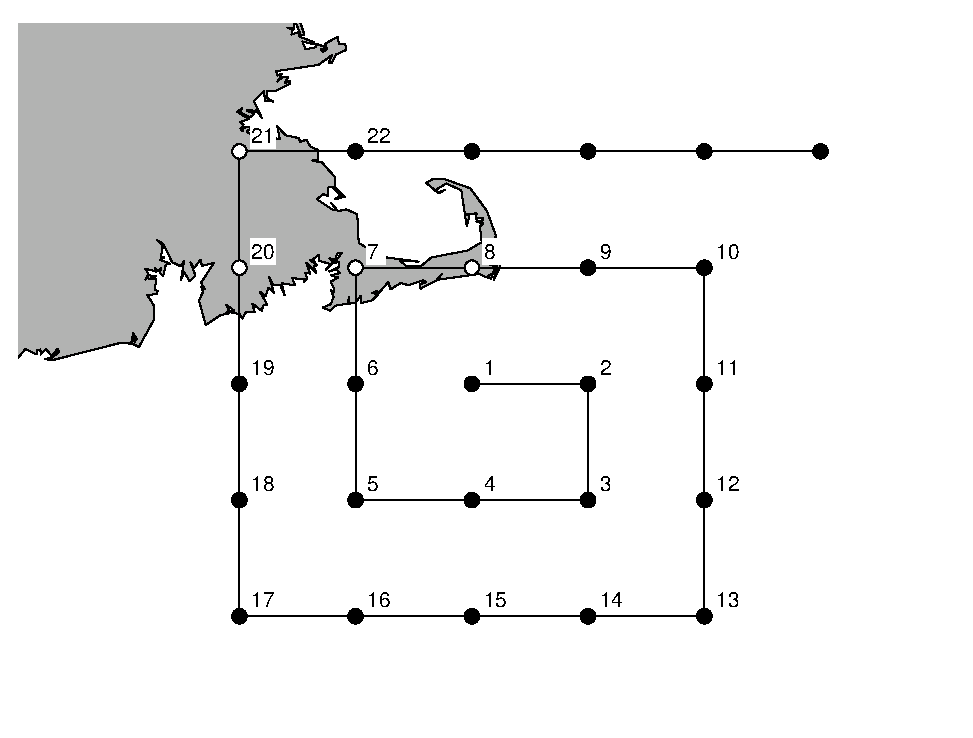
\epsfig{file=./num/wavetrack.eps,width=3.5in}
\caption{Example of a tracking spiral on a regular computational grid 
over a coastal domain featuring landmass (shaded). Black dots indicate 
active grid points and white dots indicate inactive (dry) grid points.}
         \label{fig:wavetrack} \botline
\end{center}
\end{figure}

\begin{equation}
    GoF_{i} = {\left( \frac{T_\mathrm{p} - \tilde{T}^\mathrm{n}_{\mathrm{p},i}}{\Delta T_\mathrm{n}} \right)}^2 + 
                     {\left( \frac{\theta_\mathrm{p} - \tilde{\theta}^\mathrm{n}_{\mathrm{p},i}}{\Delta\theta_\mathrm{n}} \right)}^2 +
                     {\left( \frac{H_\mathrm{m0} - \tilde{H}^\mathrm{n}_{\mathrm{m0},i}}{\Delta H_\mathrm{n}} \right)}^2\ \ ,
\label{eq:grdgof}
\end{equation} 

\noindent
where $\Delta T_\mathrm{n}$, $\Delta\theta_\mathrm{n}$ and $\Delta
H_\mathrm{n}$ are combining criteria \citep{art:WHD13}. If either of the first
two terms on the right hand side of (\ref{eq:grdgof}) exceed unity for the
closest match, the difference is considered too great and a new wave system is
assigned to that partition. Here, the search range for neighboring points is
set at 1, so that a maximum of four previously-associated neighbors can be
found (e.g. location 15 will have the previously processed neighbors 3, 4, 5
and 14). In some cases, iterative combining is required.

The next step is to correlate these wave systems over time. Each system $i$ at
the current time level $t$ is associated with its closest match amongst the
systems $j$ at the previous time level $(t-1)$. Three characteristics of the
wave systems are considered in this process, namely: (i) the spatial mean peak
wave period over the system, $\tilde{T}^\mathrm{s}_{\mathrm{p},t,i}$, with
$\mathrm{s}$ denoting the system mean, (ii) the spatial mean peak wave
direction, $\tilde{\theta}^\mathrm{s}_{\mathrm{p},t,i}$ and (iii) the number
of overlapping grid points between the two systems in geographical space
$\cap_{i,j}$. These characteristics are combined to form the following
GoF function:

\begin{equation}
    GoF_{i,j} = {\left( \frac{\tilde{T}^\mathrm{s}_{\mathrm{p},t,i} - \tilde{T}^\mathrm{s}_{\mathrm{p},t-1,j}}{\Delta T_\mathrm{s}} \right)}^2 + 
                       {\left( \frac{\tilde{\theta}^\mathrm{s}_{\mathrm{p},t,i} - \tilde{\theta}^\mathrm{s}_{\mathrm{p},t-1,j}}{\Delta\theta_\mathrm{s}} \right)}^2 +
                       {\left( \frac{N_{t-1,j} - \cap_{i,j}}{0.5N_{t-1,j}} \right)}^2\ \ ,
\label{eq:timegof}
\end{equation} 

\noindent
where $\Delta T_\mathrm{s}$ and $\Delta\theta_\mathrm{s}$ are combining
criteria, and $N$ is the total number of grid points in a system, see
\cite{art:WHD13}. In order to focus the tracking process on high-energy
regions in the wave field, the spatial mean period and peak direction values
of each system are weighted with the square of the significant wave
height. System $i$ at the current time level $t$ is assigned the system $j$
from the previous time level $(t-1)$ that minimizes (\ref{eq:timegof}). If any
of the three terms on the right hand side of (\ref{eq:timegof}) exceed unity
for the system that minimizes (\ref{eq:timegof}), a new system number is
assigned. For the last term, this implies a minimum spatial overlap
requirement, arbitrarily set at 50\%. This term mostly has an impact over
basin scale domains, where systems are typically smaller than the
computational area. In order to improve robustness, the details of identified
systems are stored for five time levels, after which the system association is
released.




\pagestyle{myheadings} \setcounter{page}{1} \setcounter{footnote}{0}

\section{~Setting up nested runs} \label{app:nest}
\newcounters 
\vssub
\subsection{~Using {\file ww3\_shel}}
\vssub

The mechanics of running nested models using the single-grid wave model
program {\file ww3\_shel} in principle is simple. A large scale model produces
a file with boundary data, for instance {\file nest1.ww3}. This file is then
renamed to {\file nest.ww3} and put in the directory in which the nested
(small scale) model is run. The small scale model then will automatically
process the file and update the boundary conditions as required and
available. Setting up the nesting consistently is more involved. A simple
step-by-step method is presented here. Another possibility, described in the
next subsection is to assemble the {\file nest.ww3} file from spectral output
using {\code ww3\_bound}.

\newcounter{nestlist}

\begin{list}{\arabic{nestlist})}{\usecounter{nestlist}
             \rightmargin 5mm \labelsep 3mm
             \labelwidth 5mm \leftmargin 10mm}

\item The first step is to set up the large scale model completely, but
      without generating boundary data for the nested model(s). Include the
      proper wind fields, graphical outputs etc. Test this model until you are
      satisfied that it works properly.

\item Set up the small scale model, for the moment ignoring the boundary
      conditions. Take into consideration that the boundary conditions ideally
      should coincide with grid lines in the large scale model to minimize the
      file size of the boundary data files. Set up this model in the same way
      as the large scale model, and test it thoroughly.

\item When the small scale model is set up satisfactorily in the above way,
      the boundary conditions need to be defined. Go into the file {\file
      ww3\_grid.inp} for the small scale model, and mark all the intended
      input boundaries as outlined in the documentation in
      section~\ref{sub:ww3grid}. Make sure that the model switch {\F !/O1} is
      selected in the {\file switch} file, and recompile if necessary. Run
      {\code ww3\_grid} and save the screen output. The output of this program
      now includes a list of all points that are marked as input boundary
      points. Also make sure that stored copies of {\file mod\_def.ww3} for
      the small scale model (if any) are properly updated.

\item The next step is to include all the input boundary points in the above
      list as output boundary points in the large scale model. Keep the list
      handy, and go to the file {\file ww3\_grid.inp} for the large scale
      model. Add all points of the above list as output boundary points as
      indicated in the documentation in section~\ref{sub:ww3grid}. Make sure
      that all data (an no other data) is sent to a single file, and run
      {\code ww3\_grid} with the proper input file. This should now give a
      list of output boundary points that should be consistent with the above
      list of input boundary points. Note that the order in which the points
      occur in the list is inconsequential. Again make sure that stored copies
      of {\file mod\_def.ww3} for the large scale model (if any) are properly
      updated.

\item If there are discrepancies between the two lists of points, iterate
      between the two previous steps until the list are consistent.

\item The next step is to start generating the boundary data from the large
      scale model. This requires the nesting output to be activated in the
      large scale model. The output is already set up and included in the
      model definition file ({\file mod\_def.ww3}) of the large scale model in
      the above steps. It now needs to be activated by setting the beginning
      time, time increment and ending time in the input file {\file
      ww3\_shel.inp} for the actual model run of the large scale model. This
      step does not need to be performed if a second or consecutive nest is
      added. The large scale model will now produce the file with boundary
      data. If this is the first nest included the output file will be {\file
      nest1.ww3}. This file needs to be saved for use in the small scale
      model.

\item To include the nesting data in the small scale model, the above boundary
      data file needs to be renamed to {\file nest.ww3} and needs to be put in
      the directory from which {\file ww3\_shel} for the small scale model is
      run. If the small scale model has properly defined the input boundary
      points in its definition file {\file mod\_def.ww3}, it will
      automatically process the file {\file nest.ww3} and update the boundary
      data as available. At this point, two additional tests are recommended.

\begin{itemize}

\item When first running the small scale model with the file {\file nest.ww3}
      present, pay close attention to the output of {\code ww3\_shel} to
      assure that (i) the program reports that the file {\file nest.ww3} has
      been processed and has been found OK, and (ii) that no additional
      warnings are present regarding incompatible or missing boundary
      data. Also check the log file {\file log.ww3} to assure that the
      boundary data are updated at the expected times.

\item When all data apparently are processed, it is illustrative and prudent to
      make a model run of the small scale model where the wind fields are
      switched off in {\file ww3\_shel.inp}, and where no restart file {\file
      restart.ww3} is made available. In such a model run, wave energy can
      only enter the domain from the boundaries. This is a good test to assure
      that the boundary data is passed from the large scale model to the small
      scale model as expected.

\end{itemize}

\end{list}

\noindent
Additional nested models can be added in the same way. Adding a second level
nest from the small scale model is also done in the same way. The model is
presently set up for producing up to 9 files with boundary data per model
run. There are no limitations on the number of consecutive (`telescoping')
nests.

\vssub
\subsection{~Using {\file ww3\_bound} and/or unstructured grids}
\vssub

In some circumstances it is difficult or impossible to know in advance the
position of the forcing points for small scale model when running the large
scale model. This is the case if one wants to run a coastal zoom using
boundary condition from an on-line or third-party database.

In this case, it is possible to generate {\file nest.ww3} file from spectral
output using {\code ww3\_bound}. This is particularly handy also for
unstructured grids due to the irregular spacing of points on the
boundary. {\code ww3\_bound} takes a list of spectra files, which should have
the same spectral grid, and generates a {\file nest.ww3}. The interpolation
coefficients are determined from the positions of the nearest available
spectra and the positions of the active boundary points in the small scale
model.

\pb
\subsection{~Using {\file ww3\_multi}}
\vssub

Performing two-way nesting in the wave model driver {\file ww3\_multi} is
greatly simplified compared to using the wave model driver {\file ww3\_shel},
because all data transfer needed is performed internally in the multi-grid
wave model routines. A mosaic model system is set up by iteratively going
through the following steps.

\begin{list}{\arabic{nestlist})}{\usecounter{nestlist}
             \rightmargin 5mm \labelsep 3mm
             \labelwidth 5mm \leftmargin 10mm}

\item Set up a grid using the {\file ww3\_grid} utility. Define the grid, its
      active boundary points and all other model information such as time
      steps, but {\it do not} attempt to generate output nesting data for
      other grids. This will be assessed automatically by the multi-grid wave
      model routines in {\file ww3\_multi}. Note that the lowest ranked grid
      can optionally use active boundary data, either as read from file or to
      be kept constant during computation. Higher ranked grids will require
      active boundary point in order to be valid in the mosaic approach,

\item Add this grid as an extra grid to the input file {\file ww3\_multi.inp}
      with the appropriate rank number. Running {\file ww3\_multi} will
      identify discrepancies between grids and requested boundary data points
      that can be resolved iteratively, and other discrepancies between grids.
      It can be tedious to remove such discrepancies by hand. The grid
      generation package of \citet{tol:MMAB07a, tol:OMOD08a} checks for such
      discrepancies automatically, and is therefore recommended for grid
      generation for this version of \ws.

\end{list}

\noindent
Note that grid on which input data fields are defined can be added in a
similar way. Note that the use of land-sea masks in oceanic input fields
(current, water level and ice) is recommended to assure realistic input values
at coastal points.

Generally, lower ranked grids are developed first, although grid of any rank
could be added at any time.

%\bpage \pagestyle{empty}


% \bpage
